\documentclass[11pt]{article}

% Prevent pdfLaTeX object-stream overflow with complex vector figures.
\ifdefined\pdfobjcompresslevel
  \pdfobjcompresslevel=0
\fi

\usepackage[letterpaper,top=0.9in,bottom=0.9in,left=0.95in,right=0.95in]{geometry}
\usepackage[T1]{fontenc}
\usepackage[utf8]{inputenc}
\usepackage{amsmath,amssymb}
\usepackage{newtxtext,newtxmath}
\usepackage{microtype}
\usepackage{graphicx}
\usepackage{booktabs}
\usepackage{tabularx}
\usepackage{array}
\usepackage{threeparttable}
\usepackage{xcolor}
\usepackage{caption}
\usepackage{float}
\usepackage{placeins}
\usepackage{titlesec}
\usepackage[numbers,sort&compress,super]{natbib}
\usepackage[colorlinks=true,citecolor=black,linkcolor=black,urlcolor=blue!55!black]{hyperref}
\usepackage{xspace}

% Cross-references to the Supplementary Information (compile supplementary.tex first).
% Long Note: Superseded by SINGLE-01; the supplement is now inline below.


% Line numbers for review copies.
% \usepackage[mathlines]{lineno}\linenumbers

\hypersetup{
  pdftitle={PangenomeFM: graph-native representation learning for human pangenomes},
  pdfauthor={Long Nguyen Tan, Tomoya Kanno, Yang Zhao, Matthew Jensen, Mark Gerstein, Yufeng Shen, Ting Wang and Xinghua Shi},
  pdfkeywords={human pangenome, graph neural network, self-supervised learning, foundation model, structural variation, regulatory genomics}
}

\newcommand{\method}{PangenomeFM\xspace}
\newcommand{\ccre}{cCRE\xspace}
\newcommand{\CI}{95\% CI\xspace}
% Items that require confirmation by the authors are shown in red.
\newcommand{\authorinput}[1]{\textcolor{red!70!black}{[#1]}}

\setcounter{secnumdepth}{0}
\titleformat{\section}{\large\bfseries}{}{0pt}{}
\titleformat{\subsection}{\normalsize\bfseries}{}{0pt}{}
\titleformat{\subsubsection}{\normalsize\itshape}{}{0pt}{}
\titlespacing*{\section}{0pt}{16pt}{6pt}
\titlespacing*{\subsection}{0pt}{12pt}{4pt}
\titlespacing*{\subsubsection}{0pt}{8pt}{3pt}
\DeclareCaptionLabelSeparator{pipe}{\ $|$\ }
\captionsetup{font=small,labelfont=bf,labelsep=pipe}
\captionsetup[figure]{name=Fig.}
\setlength{\parindent}{0.2in}
\setlength{\parskip}{1.5pt}
\widowpenalty=10000
\clubpenalty=10000
\displaywidowpenalty=10000

\makeatletter
\renewcommand{\maketitle}{%
  \begin{center}
  {\LARGE\bfseries \@title\par}
  \vspace{0.55cm}
  {\normalsize \@author\par}
  \end{center}
  \vspace{0.35cm}
}
\makeatother

% Target journal: Nature Machine Intelligence (Article).

\title{PangenomeFM: graph-native representation learning for human pangenomes}

% Long Note: HPRC and HGSVC are listed as consortium authors as requested. Their
% inclusion, position and member lists must be approved by each consortium
% before submission; member lists go in the Supplementary Information.
\author{
Long Nguyen Tan$^{1}$,
Tomoya Kanno$^{1,2}$,
Yang Zhao$^{1}$,
Matthew Jensen$^{3,4}$,
Human Pangenome Reference Consortium$^{\dagger}$,
Human Genome Structural Variation Consortium$^{\dagger}$,
Mark Gerstein$^{3,4}$,
Yufeng Shen$^{5,6}$,
Ting Wang$^{7,8}$
\& Xinghua Shi$^{1,2,*}$\\[8pt]
\small $^{1}$Department of Computer and Information Sciences, College of Science and Technology, Temple University, Philadelphia, PA, USA.
\small $^{2}$Institute for Genomics and Evolutionary Medicine, Temple University, Philadelphia, PA, USA.
\small $^{3}$Department of Molecular Biophysics and Biochemistry, Yale University, New Haven, CT, USA.
\small $^{4}$Program in Computational Biology and Bioinformatics, Yale University, New Haven, CT, USA.
\small $^{5}$Department of Systems Biology, Columbia University, New York, NY, USA.
\small $^{6}$Department of Biomedical Informatics, Columbia University, New York, NY, USA.
\small $^{7}$Department of Genetics, Washington University School of Medicine, St. Louis, MO, USA.
\small $^{8}$McDonnell Genome Institute, Washington University School of Medicine, St. Louis, MO, USA.\\[3pt]
\small $^{*}$e-mail: mindyshi@temple.edu\\[3pt]
\small $^{\dagger}$\authorinput{Proposed consortium authorship; approval and member lists pending.}
}
\date{}

% Long Note: Done [SINGLE-01]. The main text, supplement, table rows and both
% reference lists are now inline in this existing main.tex. Only figure assets
% remain external. Earlier modular files are historical and are not dependencies.
% Long Note: Done [SINGLE-02]. The supplied rewrite is edited against completed
% evidence. Findings remain out of the abstract and Introduction as requested.
% The architecture diagram introduces the model before Results; procedures are
% in Methods. The reconstruction-controls figure is supplementary to retain six
% main display items. Explicit Introduction heading follows the author's request.
% Long Note: Done [SINGLE-03]. Expanded controls and junction-development numbers
% are verified against local CSV/JSON evidence; initialization and development
% limitations are retained. No incomplete chromosome results are imported.
% Long Note: Done [SINGLE-04]. Consortium membership, grants, release hosting,
% contributions and conflicts remain author-confirmation items, not completed facts.

\begin{document}
\maketitle

% Long Note: The abstract follows the four NMI examples: problem, gap, model,
% principal findings and implication, without citations or dense numbers.
% Long Note: Superseded by SINGLE-02; the author requires an aim-focused abstract.
\begin{abstract}
Human pangenome graphs represent alternative sequence arrangements through connections among shared segments. Learning from these connections requires both genomic position and the structure of alternative routes through the graph. We introduce PangenomeFM, a self-supervised model that combines information from nearby genomic positions and connected segments through a learned gate. Pretraining predicts graph connections without biological labels. The segment representations then remain fixed when used to classify known structural variants and regulatory elements or predict locus-level susceptibility to allele-specific activity. Evaluation on held-out chromosomes compares these representations with genomic features and independently pretrained nucleotide embeddings. Graph statistics and untrained encoders provide controls for separating the contribution of graph structure from that of pretraining. The study asks whether native pangenome connectivity provides reusable biological information beyond sequence, and what learning adds to simpler graph representations.
\end{abstract}

% Long Note: Six-paragraph Introduction as requested: (1) linear to graph
% representation, (2) why representation matters biologically (Macias-Velasco et al.),
% (3) DNA foundation models, (4) topology that sequence tokens lack, (5) prior
% pangenome learning and the attribution gap, with Fig. 1 cited here and related
% work merged in, (6) PangenomeFM, its contributions and the main findings.
% Long Note: SINGLE-02 retains the contribution and study aims without findings.
\section{Introduction}
\label{sec:intro}

The human reference genome provides a coordinate system for locating genes, regulatory elements and variants. GRCh38 and the complete telomere-to-telomere CHM13 assembly are widely used for this purpose\cite{schneider2017grch38,nurk2022complete}. A single reference sequence cannot directly represent all alternative arrangements at each locus. Sequence absent from that reference must be described relative to it, complicating alignment, variant discovery and annotation in structurally diverse regions\cite{paten2017genome,eizenga2020pangenome}. Pangenome graphs represent shared and alternative sequences as connected segments, allowing different genomic arrangements to be described as routes through the graph\cite{garrison2018variation,li2020minigraph,hickey2024pangenome}. Haplotype-resolved assemblies from the Human Pangenome Reference Consortium (HPRC) and Human Genome Structural Variation Consortium (HGSVC) have made such representations increasingly practical\cite{hprc2023draft,hgsvc2021,hgsvc32025}.

Genome representation matters for both structural and functional genomics. Assembly-based pangenomes improve access to structurally diverse loci and support variant discovery\cite{hprc2023draft,hgsvc32025}; pangenome-based inference also allows known structural variants (SVs) to be genotyped across large cohorts\cite{siren2021giraffe,ebler2022pangenie}. Functional assays introduce a different set of challenges. Macias-Velasco and colleagues compared reference, personal and pangenome representations across accessibility, expression, methylation and chromatin-contact assays, showing that the effect of genome choice depends on the assay and its analysis pipeline\cite{maciasvelasco2026benchmarking}. These studies motivate a further question: whether a model can learn from the structure of a pangenome to predict biological properties beyond those already captured by nucleotide sequence and genomic position.

Genomic foundation models learn reusable features from large collections of DNA. DNABERT, DNABERT-2, HyenaDNA and the Nucleotide Transformer support regulatory and variant-related prediction\cite{ji2021dnabert,zhou2024dnabert2,nguyen2023hyenadna,dalla2025nucleotide}; related models score variants from masked-nucleotide likelihoods\cite{benegas2023gpn} or predict regulatory activity from sequence\cite{avsec2021enformer}. Although their training data can include population diversity, individual inputs are linear strings. They do not explicitly describe which alternative segments connect at a locus. Moreover, frozen sequence representations differ in their utility across tasks and do not uniformly outperform simpler regulatory baselines\cite{tang2025evaluating}. A graph representation should therefore be evaluated against a defined sequence model on the same examples, rather than presumed useful because it encodes a richer data structure.

Pangenome topology describes where alternative routes branch, where they rejoin and how their segments are oriented. Segments with similar nucleotide composition can occupy different structural contexts, while structurally similar regions can contain divergent sequences. The graph also defines a neighbourhood distinct from genomic proximity. Alternative alleles can occupy similar reference positions without being directly connected, whereas the flanks of a deletion can be distant in reference coordinates but adjacent in the graph. A representation must accommodate both relationships and their orientations. Aggregate connectivity alone does not identify which donor follows each route, however; individual allelic interpretation additionally requires verified haplotype paths.

Existing approaches introduce pangenome information at different stages of learning (Fig.~\ref{fig:paradigms}). DeepGene converts graph-derived information into sequence input\cite{zhang2025deepgene}. PangenomeX uses a phylogeny-guided network of copy-number relationships among individuals for supervised prediction\cite{xue2025pangenomex}. Learning directly from native segment connectivity without biological labels poses a different problem. Graph attention\cite{velickovic2018gat} and objectives that reconstruct connections or masked node features\cite{kipf2016vgae,hu2020strategies,hou2022graphmae} provide established tools, but link-prediction performance can depend strongly on how positive and negative examples are constructed\cite{li2023heart,dong2022fakeedge}. This is a potential form of shortcut learning\cite{geirhos2020shortcut}. Two comparisons are therefore needed: whether a graph representation adds predictive information beyond coordinates and sequence, and whether trained weights improve on graph statistics and an untrained encoder of the same design.

Here we introduce \method to learn segment representations directly from human pangenome connectivity (Fig.~\ref{fig:method}). Oriented segments retain the direction of graph connections. At each layer, a learned gate combines attention over nearby genomic positions with attention over connected segments. The model is pretrained to recover hidden connections, after which its representations remain fixed. We evaluate known SV types, candidate cis-regulatory elements (cCREs) and EN-TEx allele-specific activity\cite{rozowsky2023entex} on chromosomes excluded from downstream training. Comparisons with sequence embeddings, graph statistics and untrained encoders are designed to distinguish information present in the graph from the contribution of pretraining. Additional objectives and external evaluations test the assumptions and scope of this approach.

\begin{figure}[tbp]
  \centering
  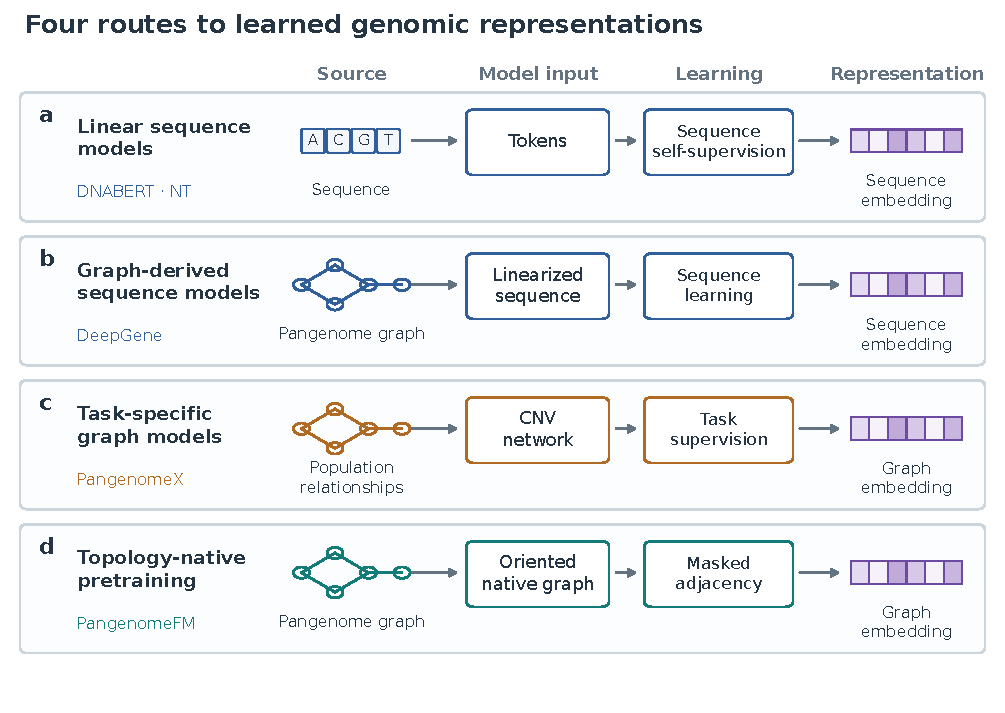
\includegraphics[width=0.92\linewidth]{figures/Fig1_paradigms.pdf}
  \caption{\textbf{Four routes from genomes to learned representations.}
  \textbf{a},~Linear sequence models, such as DNABERT and the Nucleotide Transformer (NT), tokenize nucleotide sequence and learn sequence embeddings by self-supervision.
  \textbf{b},~Graph-derived sequence models, such as DeepGene, start from a pangenome graph but convert it into linear sequences before learning.
  \textbf{c},~Task-specific graph models, such as PangenomeX, learn from a network of copy-number (CNV) relationships among individuals under supervision for a defined endpoint.
  \textbf{d},~\method learns directly from the native segment graph of a human pangenome, using oriented segments and the recovery of masked connections as the training signal, without biological labels.
  Each route ends at a learned representation, and any of them can be reused for downstream prediction. The panels compare how pangenome information enters learning, not predictive performance.}
  \label{fig:paradigms}
\end{figure}

\begin{figure}[tbp]
\centering
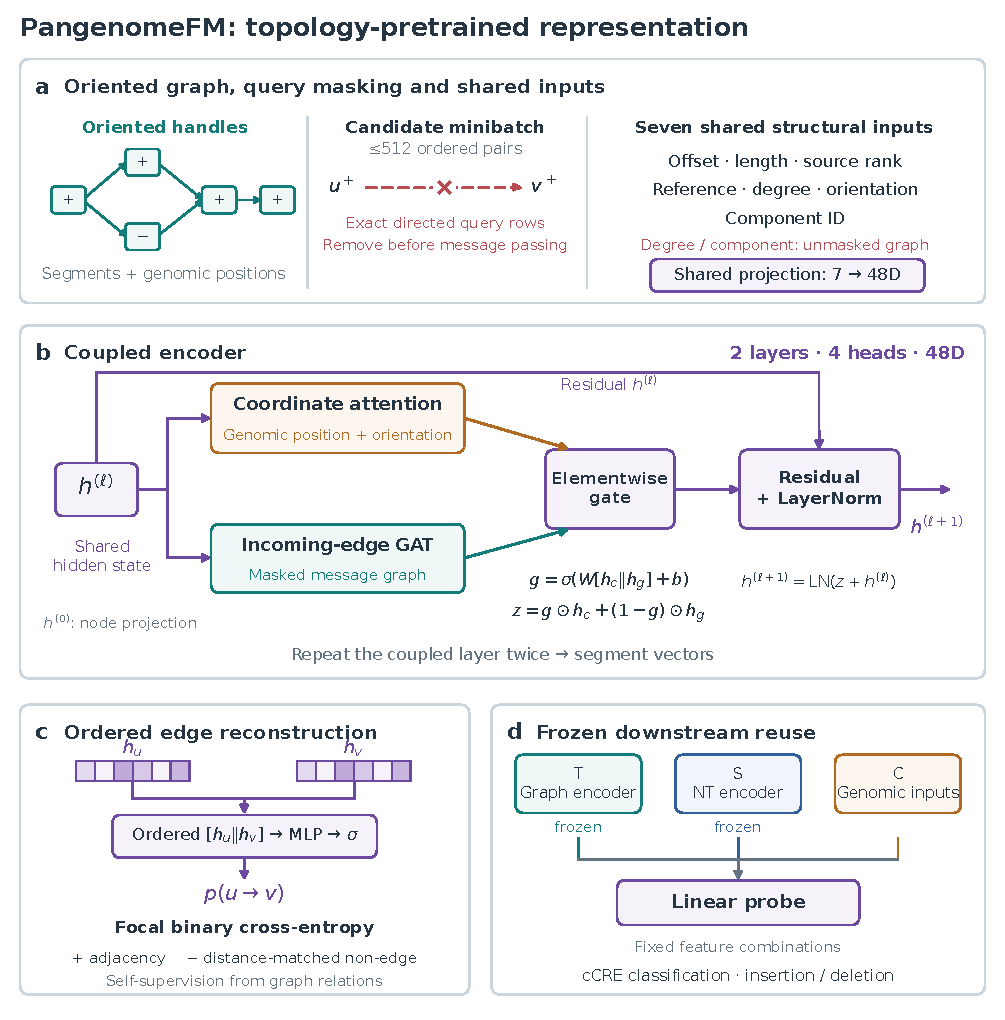
\includegraphics[width=0.9\linewidth]{figures/Fig2_architecture.pdf}
\caption{\textbf{Architecture, pretraining and frozen evaluation of \method.}
\textbf{a},~Each graph segment is represented by two oriented handles carrying seven structural descriptors derived from the graph and from genomic coordinates; no sequence or annotation is used. Connections queried in a training minibatch are removed before message passing. Connection counts and component labels are computed on the complete graph (Methods).
\textbf{b},~In each of two layers, coordinate attention over handles nearby in genomic position and graph attention over connected handles update a shared state. A per-feature gate mixes the two messages, followed by a residual connection and layer normalization.
\textbf{c},~An ordered pair scorer predicts whether a hidden connection exists and is trained with a class-weighted focal loss against pairs matched for genomic distance and connection count.
\textbf{d},~After pretraining the encoder is frozen. Graph representations ($T$), frozen Nucleotide Transformer embeddings ($S$) and genomic features ($C$) are combined in linear probes trained on chromosomes held out from evaluation; graph statistics ($H$) and untrained encoders ($R$) serve as controls.}
\label{fig:method}
\end{figure}

\FloatBarrier
\section{Results}
\label{sec:results}

% Long Note: Per the 22 September meeting and the comment asking that the first
% subsections highlight the novel components, Results opens with the design of
% PangenomeFM and its evaluation logic (Fig. 2), which the Methods then specify.
% Long Note: Superseded by SINGLE-02; Results opens with measured biological outcomes.
% Long Note: The SV section now covers SV types and stratified analyses as asked in
% the 22 September group meeting (types, allele frequency, length, complexity,
% donors), including the three-class INS/DEL/INV extension.
\subsection{Graph context improves structural-variant classification beyond sequence}
\label{sec:sv-result}

We compared genomic coordinate and structural features ($C$) and frozen Nucleotide Transformer embeddings ($S$), with or without frozen PangenomeFM representations ($T$). Performance is reported as average precision (AP), the area under the precision--recall curve. Strict graph context uses each 5-Mb region alone; one-hop context also includes directly connected segments. Only the downstream classifier receives biological labels.

We first asked whether graph representations help to distinguish types of known SVs, a task in which the local arrangement of segments should matter. Using sequence-resolved insertions and deletions of at least 50~bp from HGSVC3 mapped to the graph\cite{hgsvc32025}, we classified insertions against deletions from the representations of the segments at each event's two endpoints; only the logistic-regression classifier saw the labels. Adding $T$ to $C+S$ raised AP from 0.8721 to 0.9063 in the strict context and to 0.9122 in the one-hop context, paired gains of 0.0342 (\CI 0.0324--0.0362) and 0.0401 (0.0361--0.0440) (Fig.~\ref{fig:sv}a,b). The one-hop context added 0.0058 (0.0033--0.0084) beyond the strict context. The reciprocal contrast was null: once $C$ and $T$ were included, adding $S$ changed AP by $-0.0002$ and $-0.0005$, with intervals spanning zero. Sequence embeddings were informative on their own and improved on k-mer composition by 0.0808 (Supplementary Table~\ref{S-stab:factorial}), so the null reciprocal contrast applies to these particular features and probes; it does not establish that graph context captures all sequence information relevant to SVs.

The gain was not confined to a subset of variants. It was positive in all four allele-frequency groups and in every length group with adequate sample size, and it was largest for 50--100-bp events (0.0475 strict, 0.0547 one-hop; Fig.~\ref{fig:sv}c,d and Supplementary Table~\ref{S-stab:svlength}). Events of 100~kb--1~Mb, with about 27 test examples per run, gave negative but highly uncertain estimates, which we report rather than exclude. We expected graph context to help most where the graph is most complex, but the trend ran the other way. With a complexity score fixed before any model was evaluated (Methods), strict gains were 0.0419, 0.0380 and 0.0302 in low-, medium- and high-complexity regions, and one-hop gains were 0.0499, 0.0474 and 0.0336 (Supplementary Fig.~\ref{S-sfig:complexity}). The high-minus-low differences were $-0.0117$ ($-0.0230$ to $-0.0019$) and $-0.0162$ ($-0.0267$ to $-0.0092$), although exact fold-level tests could not resolve them ($P=0.125$ and $P=0.0625$). Finally, because HGSVC3 and HPRC share at least five donors, we stratified test events by carrier. Excluding the shared donors, the mean gain across the remaining 60 donors was 0.0367 (0.0339--0.0395) strict and 0.0430 (0.0393--0.0470) one-hop (Supplementary Fig.~\ref{S-sfig:donor}). Classifiers were still trained on these donors' variants from other chromosomes, so this analysis addresses donor overlap between resources rather than generalization to unseen individuals.

\begin{figure}[tbp]
  \centering
  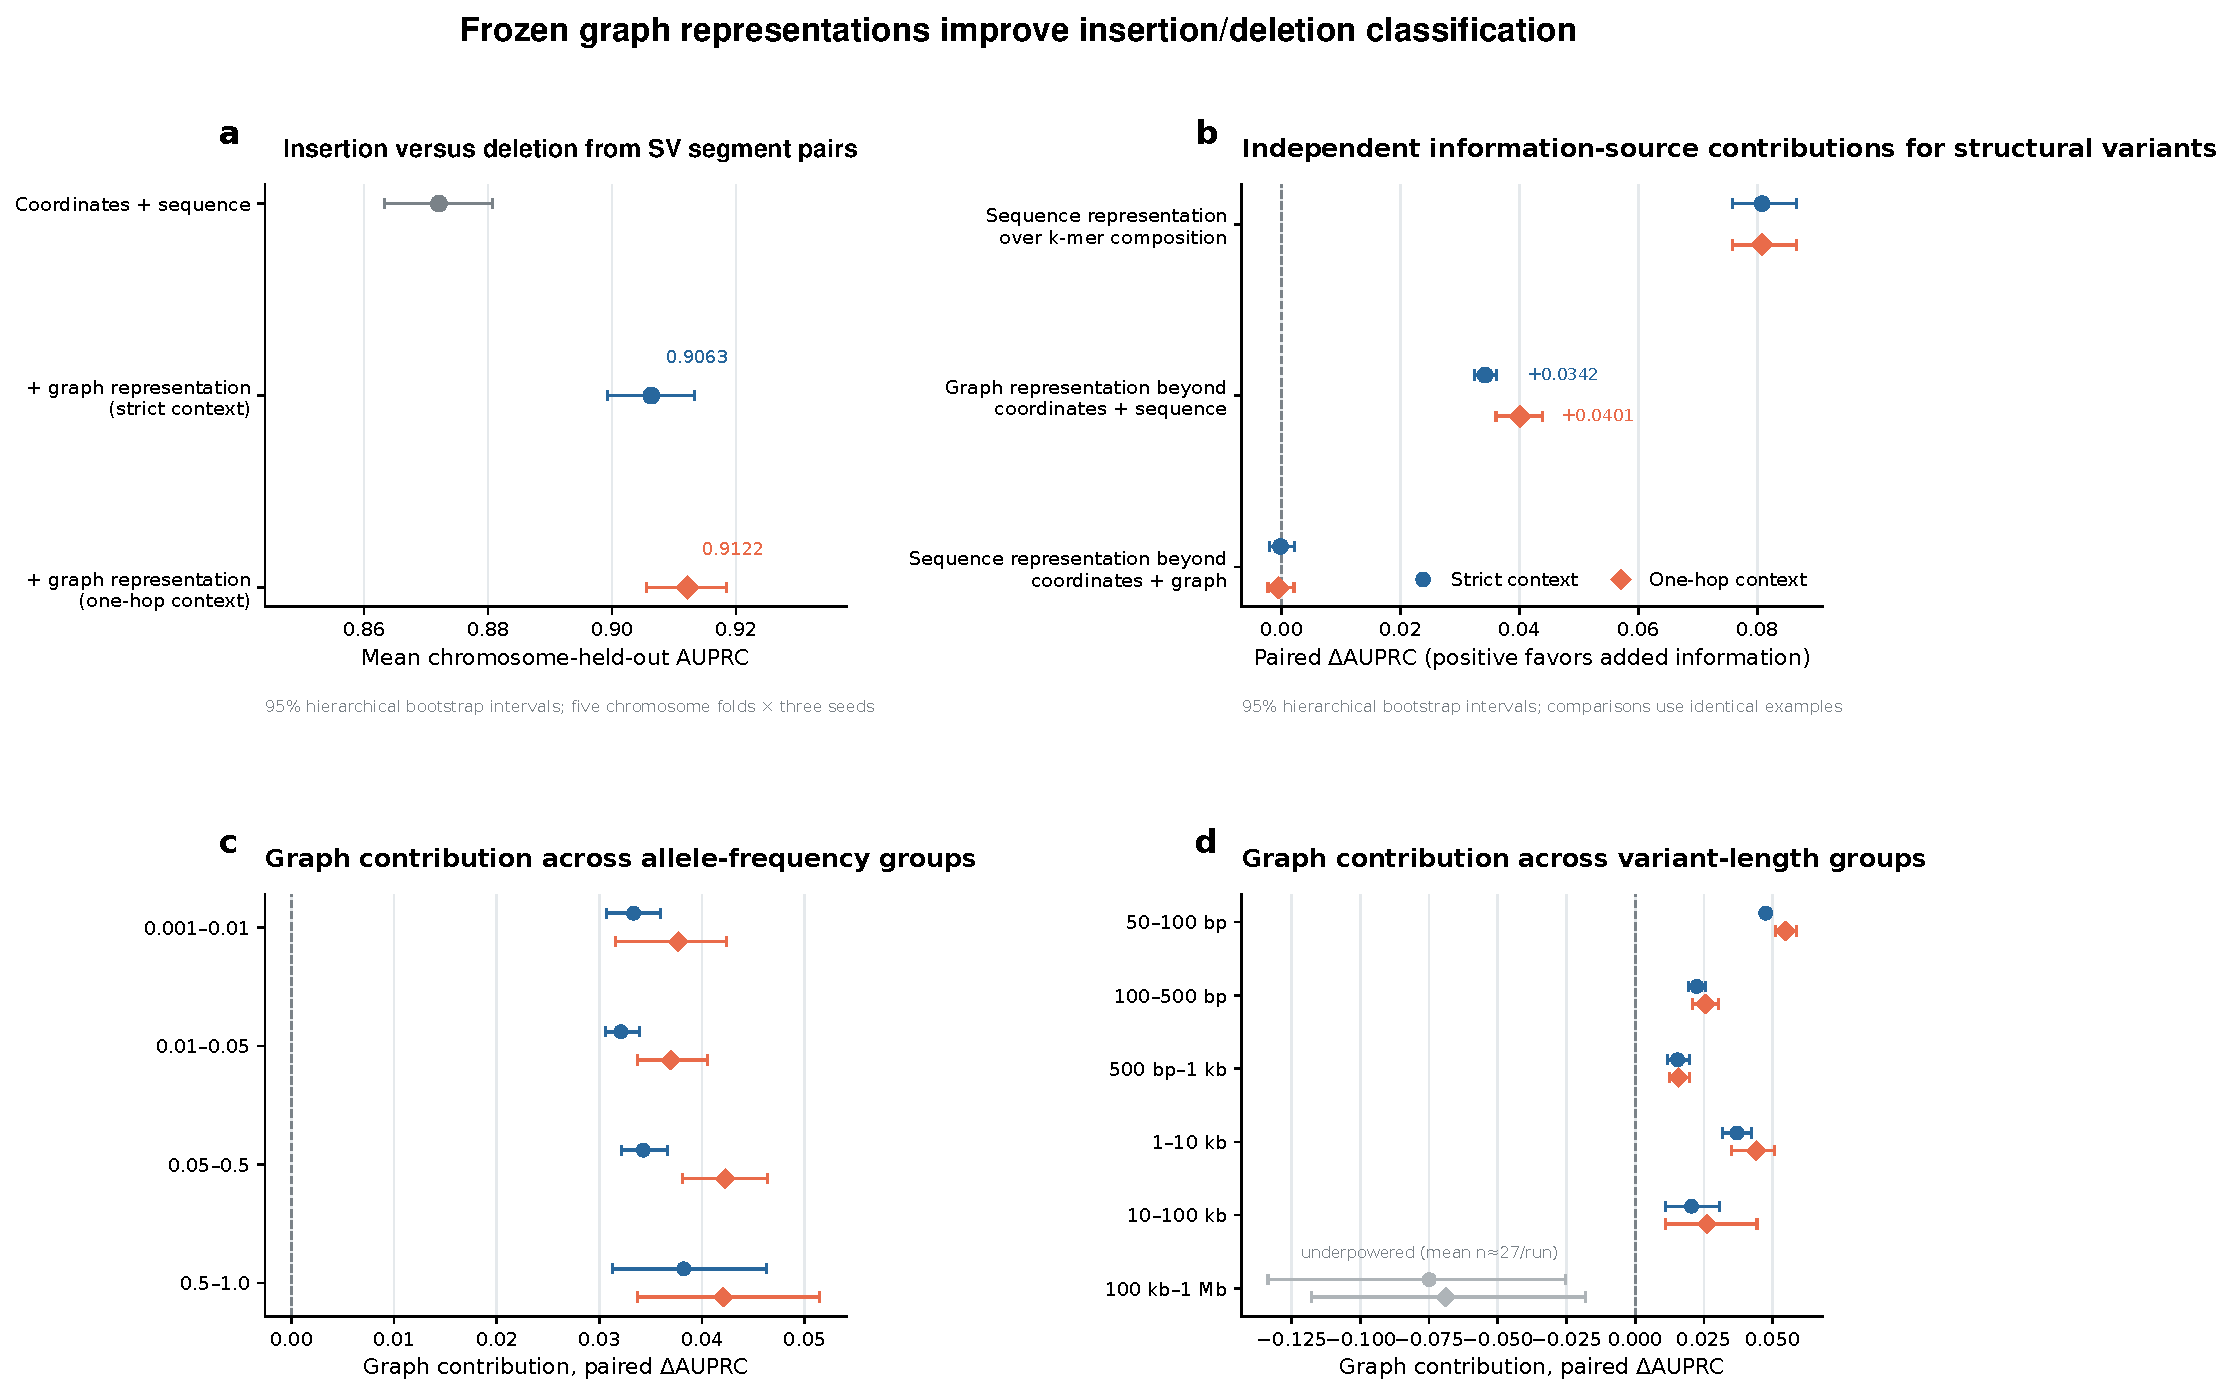
\includegraphics[width=\linewidth]{figures/Fig3_structural_variants.pdf}
  \caption{\textbf{Graph representations improve structural-variant classification.}
  \textbf{a},~Held-out-chromosome AP for classifying insertions against deletions using genomic features and sequence embeddings ($C+S$), and after adding frozen \method representations under strict and one-hop context.
  \textbf{b},~Paired contrasts on identical examples: sequence embeddings over k-mer composition, graph representations beyond $C+S$, and sequence embeddings beyond $C+T$. Positive values favour the added information.
  \textbf{c},\textbf{d},~Graph contribution beyond $C+S$ by allele-frequency group (\textbf{c}) and SV length (\textbf{d}). The 100~kb--1~Mb group (about 27 test events per run) is underpowered and shown in grey.
  Points show means over five chromosome folds and three pretraining runs; bars show 95\% hierarchical bootstrap intervals.}
  \label{fig:sv}
\end{figure}

% Long Note: Kept the controlled multiclass result in the main text, with the
% uncertain inversion result and the absent random-encoder arm stated explicitly.
% Run counts, convergence checks and the common-support sensitivity are in
% Supplementary Note 4.
\subsubsection{A three-class extension tests whether the signal persists beyond insertions and deletions}
\label{sec:sv-type-extension}

Insertions and deletions differ in length and in simple local statistics, and a classifier can exploit both. To ask whether the graph representation carries information beyond these properties, we extended the task to three classes by adding inversions and represented each event by the segment containing its first affected base. We retained all 174,267 primary-chromosome events at their observed frequencies (110,623 insertions, 63,346 deletions and 298 inversions) and fitted a one-versus-rest classifier for each class. Adding $T$ to $C+S$ increased macro AP, the unweighted mean of the three one-versus-rest APs, from 0.4070 to 0.4740 in the strict context and to 0.4586 in the one-hop context (Table~\ref{tab:sv-natural}). When measured event log length ($L$) and 14 label-free graph statistics ($H$) were also included, $T$ still added 0.0477 (0.0399--0.0553) and 0.0150 (0.0077--0.0214).

The macro gain did not establish a benefit for inversions specifically. With 298 inversions, the inversion-specific gains after $L$ and $H$ had intervals that included zero in both contexts. This extension also lacks an untrained-encoder arm, so it shows that $T$ carries information beyond length and graph statistics without showing that the information was learned. In a sensitivity analysis that matched chromosome and length distributions across classes (223 events per class), the gain from adding $T$ after $H$ was inconclusive (Supplementary Note~\ref{S-snote:threeclass}). For the natural-frequency macro contrasts, exact fold-level sign-flip tests reached their minimum attainable value ($P=0.0625$; Benjamini--Hochberg $q=0.0741$ within the metric), so the positive bootstrap intervals should be read as pointwise evidence. All estimates describe the ascertained HGSVC3 call set rather than population SV frequencies.

\begin{table}[tbp]
\centering
\caption{\textbf{Three-class SV classification at natural class frequencies.} Mean AP over five chromosome folds and three pretraining runs per context, before and after adding frozen graph representations ($T$) to the stated baseline. Macro AP is the unweighted mean of the insertion, deletion and inversion one-versus-rest APs; the inversion class contains 298 of 174,267 events. $L$, measured event log length; $H$, 14 graph statistics. Intervals are pointwise 95\% hierarchical bootstrap intervals.}
\label{tab:sv-natural}
\footnotesize
\setlength{\tabcolsep}{4pt}
\begin{tabular}{@{}lllrrrl@{}}
\toprule
Endpoint & Context & Baseline & Baseline AP & Baseline $+T$ AP & $\Delta_T$ & 95\% CI \\
\midrule
Macro AP & Strict & $C+S$ & 0.4070 & 0.4740 & 0.0671 & 0.0623 to 0.0708 \\
Macro AP & One-hop & $C+S$ & 0.4070 & 0.4586 & 0.0517 & 0.0473 to 0.0553 \\
Macro AP & Strict & $C+S+L+H$ & 0.5082 & 0.5558 & 0.0477 & 0.0399 to 0.0553 \\
Macro AP & One-hop & $C+S+L+H$ & 0.5082 & 0.5232 & 0.0150 & 0.0077 to 0.0214 \\
Inversion AP & Strict & $C+S$ & 0.0069 & 0.0089 & 0.0019 & 0.0007 to 0.0031 \\
Inversion AP & One-hop & $C+S$ & 0.0069 & 0.0091 & 0.0022 & 0.0017 to 0.0028 \\
Inversion AP & Strict & $C+S+L+H$ & 0.1743 & 0.1895 & 0.0152 & $-$0.0043 to 0.0365 \\
Inversion AP & One-hop & $C+S+L+H$ & 0.1743 & 0.1728 & $-$0.0015 & $-$0.0197 to 0.0117 \\
\bottomrule
\end{tabular}
\end{table}

% Long Note: cCRE and ENCODE results as requested (binary cCRE, PLS/pELS/dELS/CTCF-only
% and complexity strata), followed by EN-TEx activity (1-1 meeting, 11 September).
\subsection{Graph and sequence representations are complementary for regulatory elements}
\label{sec:ccre-result}

Regulatory elements pose a different problem. Whether a segment overlaps a cCRE depends largely on its sequence, and graph structure might add context about the surrounding variation. For classification of ENCODE cCREs against background segments\cite{encode2020registry}, $C+S$ reached AP 0.9185, and adding $T$ increased it to 0.9225 (strict) and 0.9219 (one-hop), paired gains of 0.0040 (0.0029--0.0048) and 0.0034 (0.0017--0.0048) (Fig.~\ref{fig:ccre}a,b). Here the balance between the two sources reversed relative to SVs. Sequence embeddings improved on k-mer composition by 0.3151 and still added 0.0248 and 0.0261 beyond $C+T$ (Supplementary Table~\ref{S-stab:factorial}). Within predefined ENCODE classes, each compared with the common background using the same classifier, strict gains were 0.0058 for promoter-like elements, 0.0209 for proximal enhancer-like elements, 0.0054 for distal enhancer-like elements and 0.0349 for CTCF-only elements (Fig.~\ref{fig:ccre}c). In contrast to SVs, the gain was largest in high-complexity regions (0.0076, compared with 0.0018 and 0.0014 in low- and medium-complexity regions; Fig.~\ref{fig:ccre}d). These subgroup results come from a single classifier and are descriptive.

We next asked whether graph context helps to predict measured regulatory activity rather than annotation. EN-TEx provides personal epigenomes and allele-specific (AS) measurements across tissues from four individuals\cite{rozowsky2023entex}. Because \method assigns one vector to each segment, these tasks test whether a locus is prone to AS activity, not which allele is favoured in a given person. The contribution of $T$ depended on the assay (Supplementary Table~\ref{S-stab:entex}). Predicting which cCREs are prone to AS activity was inconclusive in both contexts (strict gain 0.00021, $-0.00032$ to 0.00075), as was classifying distal enhancer-like elements as active or repressed, averaged over five tissues. For AS single-nucleotide variants (SNVs), CTCF binding gave small positive gains of 0.00147 (0.00010--0.00355) strict and 0.00225 (0.00096--0.00348) one-hop. H3K4me3 gave positive intervals in both contexts and H3K27ac in the one-hop context only, whereas RNA allele-specific expression, ATAC-seq accessibility and H3K27me3 were inconclusive. These intervals are not adjusted across the assay panel, and absolute AP was low (0.025--0.10 for the SNV endpoints), in line with the rarity of AS events. The small positive estimates and inconclusive endpoints limit a broad claim about regulatory transfer.

\begin{figure}[tbp]
  \centering
  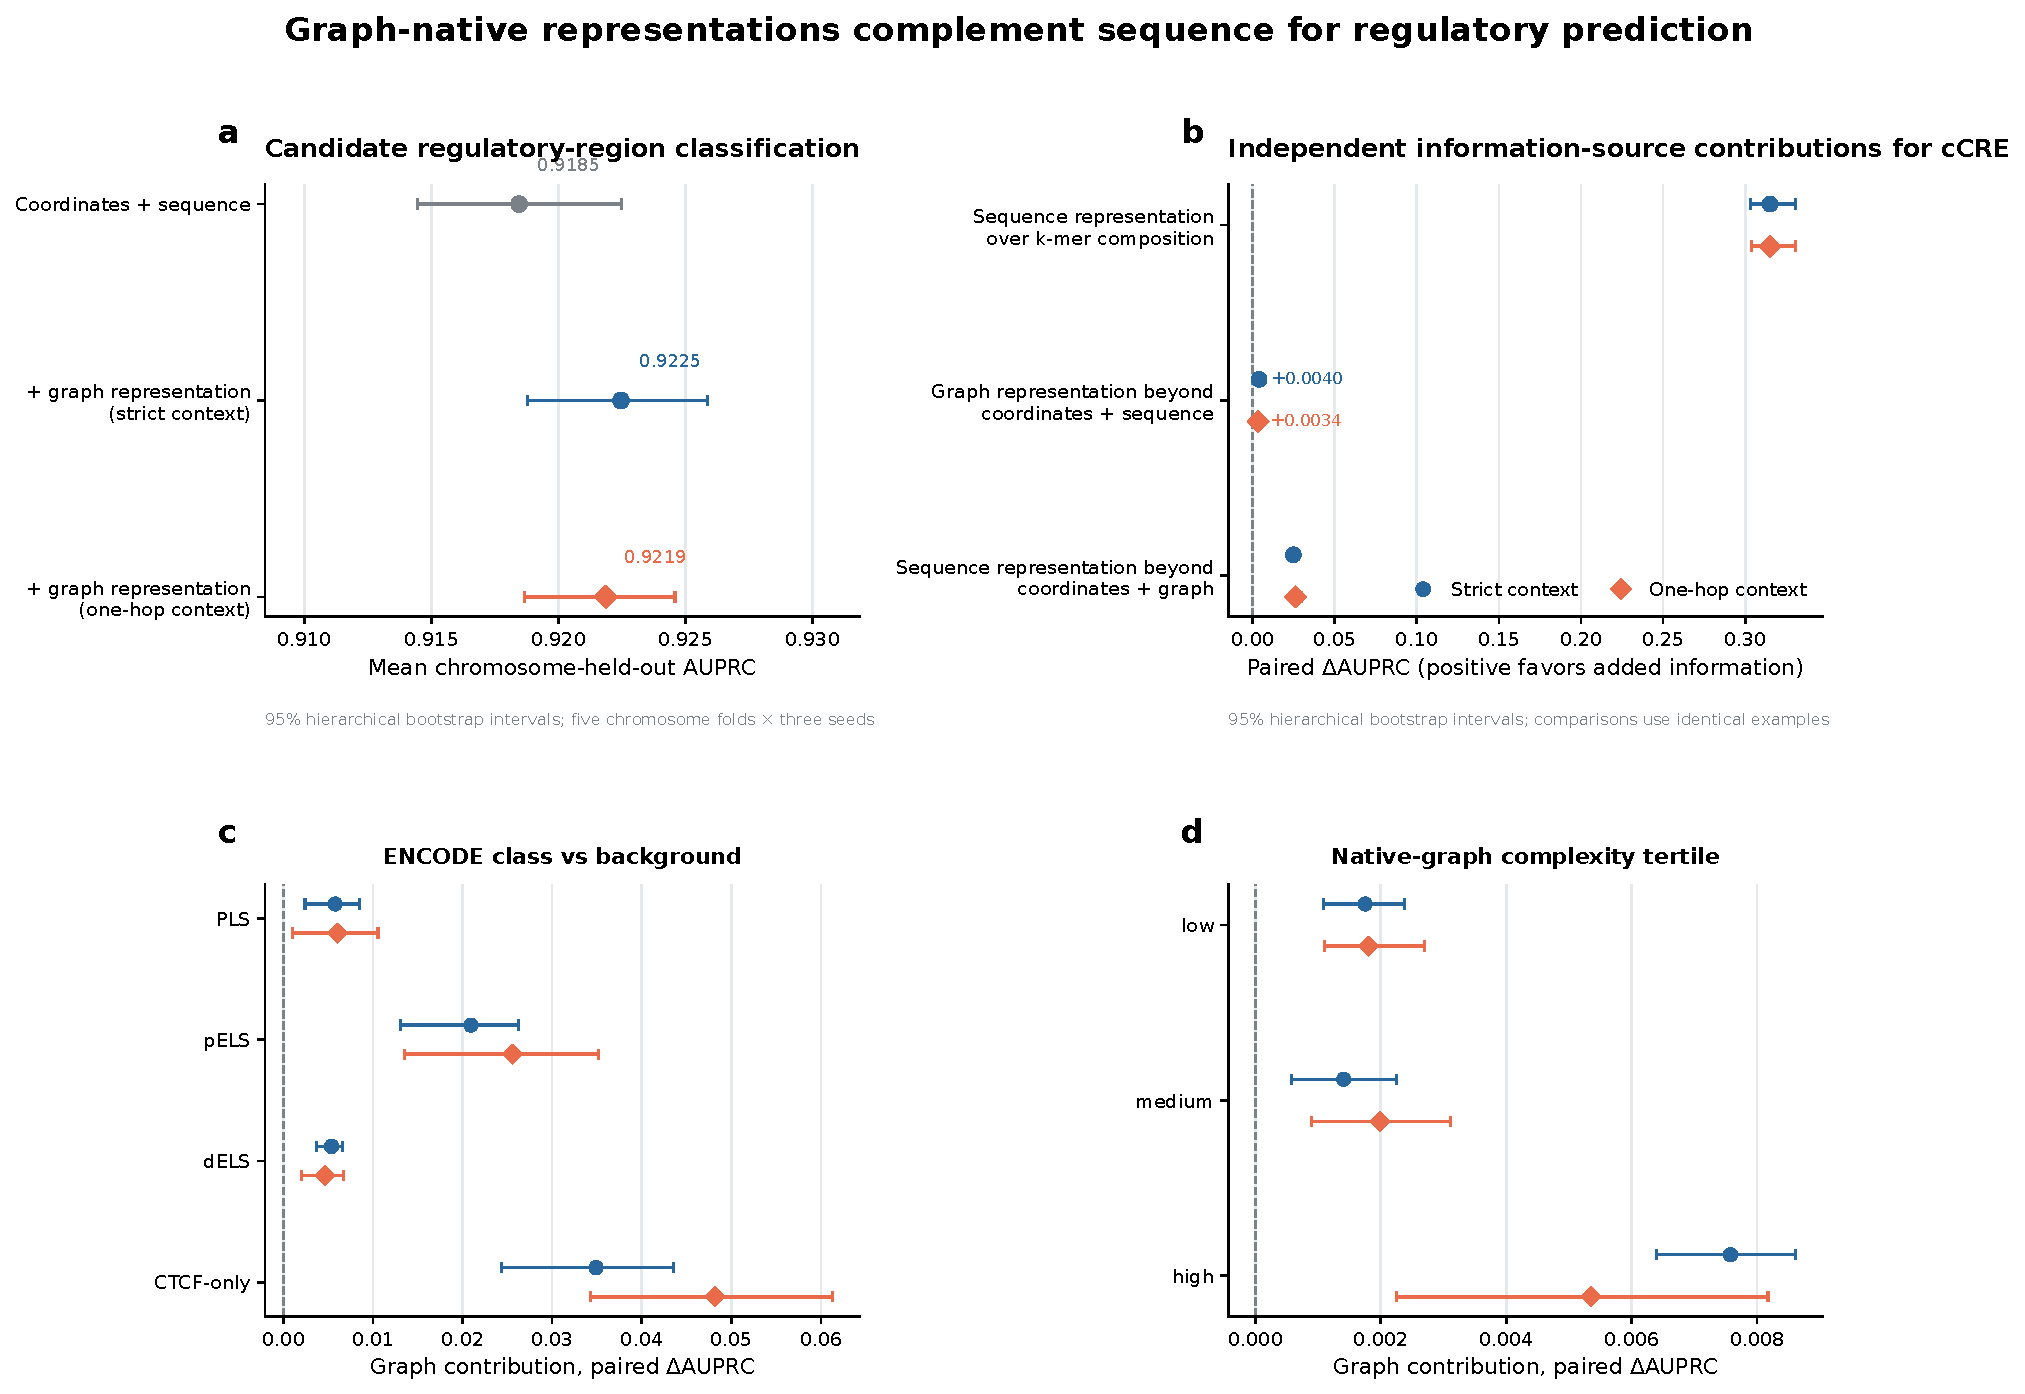
\includegraphics[width=\linewidth]{figures/Fig4_regulatory_elements.pdf}
  \caption{\textbf{Graph and sequence representations are complementary for cCRE classification.}
  \textbf{a},~Held-out-chromosome AP for classifying ENCODE cCREs against background segments using $C+S$, and after adding frozen \method representations under strict and one-hop context.
  \textbf{b},~Paired contrasts on identical examples, as in Fig.~\ref{fig:sv}b. Sequence embeddings dominate, and graph representations add a smaller, consistent increment.
  \textbf{c},~Graph contribution for ENCODE classes (promoter-like, PLS; proximal and distal enhancer-like, pELS and dELS; CTCF-only), each against the common background, evaluated from the same binary classifier.
  \textbf{d},~Graph contribution by native graph-complexity group, with thresholds fixed before model evaluation.
  Points show means over five chromosome folds and three pretraining runs; bars show 95\% hierarchical bootstrap intervals.}
  \label{fig:ccre}
\end{figure}

% Long Note: Separate Results subsection on the sequence embeddings, as requested,
% with its interpretation; quality-control details are in Supplementary Note 5.
\subsection{Sequence embeddings cover every segment, but not every nucleotide}
\label{sec:sequence-coverage-result}

Because the conclusions above depend on how well $S$ represents each segment, we examined its coverage directly. The frozen Nucleotide Transformer produced a 512-dimensional vector for every one of the 303,425 segments used by the cCRE and SV classifiers, so no example was lost for lack of sequence features. However, 26.3\% of these segments exceeded the model's input limit and were represented by equal-length samples from their two ends, up to 6,000 bases in total. For these segments the sequence model saw only part of the nucleotide content. This affects the interpretation of the SV results in particular: a sequence baseline that read complete segments might narrow the gap to $T$, and the null value of $\Delta_{S\mid C,T}$ should be read as a property of this sequence representation rather than of sequence information in general. The same sampling removes most tested variant bases in external variant benchmarks (see below). We have since embedded all 751,237 graph segments with the same model, which makes sequence available to graph models throughout the graph (Supplementary Note~\ref{S-snote:coverage}).

% Long Note: Retitled from the CS-heavy heading. The trained-versus-random table
% moves to the main text because it qualifies the central claim.
\subsection{Much of the graph contribution does not require pretraining}
\label{sec:controls-result}

A positive $\Delta_{T\mid C,S}$ shows that a representation is useful; it does not show that pretraining is responsible. The same information might be available from simple summaries of the graph, or from any network that aggregates features over the graph, whether trained or not. We therefore repeated both binary tasks with two controls: $H$, 14 label-free statistics computed from the complete graph, and $R$, an untrained encoder with the same architecture, inputs and extraction procedure as \method (Table~\ref{tab:controls}).

Graph statistics alone accounted for a large part of the SV gain. Adding $H$ to $C+S$ raised insertion-versus-deletion AP from 0.8721 to 0.9069, comparable to the gain from $T$, yet $T$ still added 0.0154 (0.0140--0.0168) strict and 0.0109 (0.0085--0.0131) one-hop beyond $C+S+H$. The untrained encoder, however, added 0.0101 and 0.0105 beyond $C+S+H$, about two-thirds of the trained increment in the strict context and nearly all of it in the one-hop context. Conditional on $C+S+H$, the trained-minus-untrained difference was 0.0053 (0.0028--0.0105) for SVs in the strict context and close to zero in the one-hop context. For cCREs it favoured the untrained encoder in the strict context ($-0.0008$; $-0.0015$ to $-0.0001$) and was inconclusive in the one-hop context. Without $H$, the trained encoder exceeded the untrained one by 0.0110 (0.0072--0.0201) for strict SVs but not in the other three settings. With five chromosome folds the exact sign-flip test cannot fall below $P=0.0625$, and no trained-versus-untrained contrast survived correction for multiple comparisons.

These controls change what the SV and cCRE results mean. The information that $T$ adds to sequence is reproducible and exceeds what 14 hand-crafted statistics capture, but most of it is obtained by passing the same structural descriptors through an untrained network of the same design. The comparison limits attribution of the observed benefit to pretraining. Probing studies of language models reached a similar conclusion, that a probe's accuracy must be compared with control conditions before it is attributed to learned structure\cite{hewitt2019control}, and the result led us to examine what the pretraining objective rewards.

\begin{table}[tbp]
\centering
\caption{\textbf{Trained versus untrained graph encoders after graph statistics.} AP increments from adding the trained encoder ($T$) or an untrained encoder of identical architecture ($R$) to $C+S+H$, and their paired difference, over 15 fold--run pairs per row. $P$ and $q$ refer to the trained-minus-untrained difference: $P$, exact two-sided sign-flip test on five fold-level differences (minimum attainable value 0.0625); $q$, Benjamini--Hochberg adjustment within the metric across the declared control contrasts. These are exploratory comparisons on previously evaluated folds. $H$ is computed on the complete graph and therefore sees a wider neighbourhood than the regional encoders. INS, insertion; DEL, deletion.}
\label{tab:controls}
\footnotesize
\setlength{\tabcolsep}{3.5pt}
\begin{tabular}{@{}llllllr@{}}
\toprule
Task & Context & $T$ after $C+S+H$ & $R$ after $C+S+H$ & Trained $-$ untrained & $P$ & $q$ \\
\midrule
INS vs DEL & Strict & 0.0154 (0.0140 to 0.0168) & 0.0101 (0.0055 to 0.0128) & 0.0053 (0.0028 to 0.0105) & 0.0625 & 0.079 \\
 & One-hop & 0.0109 (0.0085 to 0.0131) & 0.0105 (0.0063 to 0.0129) & 0.0004 ($-$0.0023 to 0.0052) & 0.875 & 0.875 \\
cCRE & Strict & 0.0027 (0.0020 to 0.0034) & 0.0035 (0.0024 to 0.0045) & $-$0.0008 ($-$0.0015 to $-$0.0001) & 0.0625 & 0.079 \\
 & One-hop & 0.0022 (0.0005 to 0.0037) & 0.0023 (0.0011 to 0.0035) & $-$0.0001 ($-$0.0009 to 0.0009) & 0.8125 & 0.848 \\
\bottomrule
\end{tabular}
\end{table}

% Long Note: This subsection reports the shortcut audit, including the visible-graph
% recomputation of degree baselines under each context (the high-priority control
% requested in the original comments), and the development of objectives that
% remove the shortcut.
\subsection{Recovering hidden connections can be solved from connection counts}
\label{sec:shortcut-result}

On its own pretraining task \method appeared highly accurate, recovering hidden connections on held-out chromosomes with AP 0.9501 in the strict context and 0.9880 in the one-hop context, against a chance level of about 0.50 (Supplementary Fig.~\ref{S-sfig:controls}a and Supplementary Note~\ref{S-snote:reconstruction}). Simple baselines told a different story. Scoring each candidate pair by the product of its endpoints' visible connection counts, the classical preferential-attachment score\cite{barabasi1999emergence,libennowell2007link}, reached 0.9835 in the strict context, above the model, and the sum of the counts reached 0.9742. Genomic coordinates (0.7003) and k-mer composition (0.6555) were far weaker.

Hiding a true connection reduces the number of visible connections at its endpoints, whereas endpoints of matched negative pairs need not lose any. The encoder also receives connection counts from the complete graph, making this difference potentially detectable without learning which segments belong together. Under one-hop context, the model exceeded preferential attachment across all complexity groups, but the additional context changes both the model inputs and the baselines. The reversal does not establish that the shortcut is removed. Recomputing the baselines on the visible graph reproduced the reported scores (Supplementary Note~\ref{S-snote:reconstruction}).

Removing graph attention reduced strict reconstruction AP to 0.7855. Larger models and more training regions improved reconstruction in some settings, but biological prediction did not improve consistently (Supplementary Notes~\ref{S-snote:reconstruction} and~\ref{S-snote:scaling}). The 96-dimensional, four-layer model reached fold-pooled AP 0.9876, compared with 0.9423 for the principal model; these fold-pooled values differ from the region-averaged headline scores.

Junction re-pairing balanced positive and negative endpoint exposure and matched their signed genomic geometry. On one development partition, geometry and degree controls scored near chance (AP 0.500--0.507). In the tested configuration, incoming-only message passing reached AP 0.501, compared with 0.503 for an untrained encoder, whereas bidirectional messages reached 0.790 versus 0.626. Sequence-conditioned variants reached 0.841 and 0.870 with different pair scorers (Supplementary Fig.~\ref{S-sfig:objectives}). These are design-selection results, not independent chromosome tests. The junction representation met the three-run biological development criterion in only one run. A separate masked sequence-feature objective\cite{hou2022graphmae} gave positive trained-minus-untrained increments after $C+S+H$ in both tasks in all three development runs (Supplementary Note~\ref{S-snote:objectives}). Neither objective has a complete chromosome-level biological result in this evidence package.



% Long Note: The genotyping question (improve SV genotyping in complex/CNV regions)
% is addressed with the COSIGT analysis; improved genotype calls are NOT shown and
% the text says so.
\subsection{External evaluations delimit the scope of reuse}
\label{sec:generalization-result}

Finally, we asked whether the representation helps with endpoints beyond the tasks on which it was characterized. For 69 clonal insertions and deletions in the HG008 genome, which was not used to train any classifier, adding $T$ to $C+S$ gave gains of 0.0325 ($-0.0534$ to 0.1103) strict and 0.0649 ($-0.0667$ to 0.2121) one-hop; with so few events the external benefit is unresolved. On TraitGym\cite{benegas2025traitgym}, which comprises 14,780 variants (11,400 complex-trait and 3,380 Mendelian) in matched groups of one putatively causal variant and nine controls, no topology contrast had a positive interval, either for a locus-level prior or when published allele scores were added (Supplementary Note~\ref{S-snote:external}). Two features of our design limit this test: the representation assigns one vector to each segment and is therefore blind to the tested allele, and end sampling left only 23--28\% of tested variant bases in the sequence input.

Improved SV genotyping, particularly in complex and copy-number-variable regions, is a natural application for pangenome representations. As a first test, we asked whether $T$ predicts where pangenome-based genotyping succeeds, using published COSIGT results at 265 complex loci\cite{bolognini2026cosigt} and a per-locus summary of call quality as the target. No fitted model outperformed a constant equal to the training-set median (mean absolute error 0.0462, compared with 0.0534 for $C+S$ and 0.0527 and 0.0538 for $C+S+T$ in the strict and one-hop contexts), and no reduction in error from adding $T$ was established in either context (intervals spanned zero). This endpoint measures call quality at loci the published pipeline could evaluate. It does not test whether \method representations would change genotype calls, which requires genotype truth, a defined set of callable loci and separate evaluation in complex regions. Reconstruction transfer between graph resources and releases, which is affected both by the degree shortcut and by shared donors, is reported in Supplementary Note~\ref{S-snote:reconstruction}.

\FloatBarrier
\section{Discussion}
\label{sec:discussion}

Learning from a human pangenome requires a distinction between where a sequence lies and how it connects to alternative sequence arrangements. \method combines these two forms of context while retaining segment identifiers that link the graph to biological annotations. Freezing the encoder before biological evaluation separates representation learning from task-specific fitting. The methodological contribution lies in this use of native pangenome connections and genomic position; it does not require treating established attention or optimization operations as new algorithms.

The biological interpretation depends on the prediction target. Classifying a known structural variant asks how an ascertained event relates to graph structure; it does not test whether the model can discover that event or genotype it in a new individual. Likewise, identifying a regulatory element and predicting its measured activity are different questions. These distinctions are essential when assessing reuse across tasks. Graph complexity can describe the setting in which a prediction is made, but neither a complex region nor an association between complexity and a label establishes a biological mechanism.

A second distinction concerns the source of predictive information. Adding a graph representation to sequence features tests whether the representation is useful. Comparing trained and random-weight encoders with the same inputs measures the additional contribution of pretraining under those controls. A reconstruction objective must also be checked for cues introduced by the masking procedure itself. These controls are necessary before attributing biological performance to learned graph relationships or describing a representation as a broadly effective foundation model. Junction re-pairing and masked-feature objectives address specific limitations of connection recovery; their biological value requires evaluation beyond the chromosomes used to choose them.

Several features of the study design limit the scope of inference. Holding out chromosomes does not hold out donors, and donors shared between graph resources complicate transfer between them. Sampling the ends of long segments restricts the context available to the sequence baseline. Aggregate graph segments lack donor paths and assign the same vector to both alleles at an SNV, preventing a direct interpretation of individual allelic effects. Insertion endpoint conventions and SV ascertainment further constrain the target population. Stronger sequence baselines, verified correspondence between segments and haplotypes, and donor-independent graphs are needed to address these limitations. Demonstrating improved genotyping would additionally require genotype truth, a defined set of callable loci and explicit evaluation in complex and copy-number-variable regions.

Further model development should therefore be judged by biological prediction beyond matched random encoders, graph statistics and sequence baselines. Comparisons must control the inputs and model capacity and reserve evaluation chromosomes from development decisions. This provides a testable criterion for improving pangenome representations: learning should improve held-out biological prediction beyond fixed graph summaries and sequence features.

% Long Note: Methods open with the novel components (graph representation,
% coupled encoder, pretraining objective with loss and optimization, frozen
% reuse and attribution design, shortcut-resistant objectives), followed by
% resources, tasks and statistics, as requested in the comments and the
% 22 September meeting.
\section{Methods}
\label{sec:methods}

\subsection{Graph representation of pangenome segments}
\label{sec:representation}

\textbf{Graph resource.} We used the structural-variant-resolution graph of HPRC release~2, distributed in reference GFA (rGFA) format\cite{li2020minigraph}, in which each segment carries a stable source name (SN), an offset on that source (SO) and a source rank (SR; 0 for GRCh38). The graph contains 751,237 segments and 1,097,658 links, every segment has complete SN, SO and SR tags, and 305,572 segments are tagged as GRCh38 sequence. The graph stores no haplotype paths, so the number of contributing genomes cannot be read from the graph itself. Haplotype paths extracted from the full-resolution graphs of the same resources comprise 454 haplotypes from 227 individuals (HPRC release~2) and 122 haplotypes from 61 individuals (HGSVC3) (Supplementary Table~\ref{S-stab:paths}). % Long Note: confirm against the HPRC release documentation which assemblies were used to build the SV-resolution graph.
Graph tables were generated from GFA and GBZ files with the variation-graph toolkit\cite{garrison2018variation,siren2022gbz}. We partitioned primary chromosomes into non-overlapping 5-Mb regions and retained 608 regions for analysis.

\textbf{Oriented handles.} Each segment $s$ is represented by two handles, $2s+o$, where $o\in\{0,1\}$ denotes forward or reverse orientation. A directed link $(u,v)$ between handles and its reverse-complement traversal $(\bar v,\bar u)$, where $\bar u$ flips the orientation of $u$, describe the same junction read on opposite strands.

\textbf{Structural inputs.} Each handle $v$ receives a seven-dimensional input $x_v$: genomic offset (SO), segment length, source rank (SR), GRCh38 membership, number of connections (degree) at that handle, orientation and connected-component index. Offset, length and degree are transformed by $\log(1+|x|)$ and divided by the largest transformed value in the region; source rank and component index are min--max scaled within the region, with constant columns set to zero; membership and orientation are binary. Degree and component index are computed on the complete graph before any connection is hidden. No nucleotide sequence or biological label enters the encoder.

\textbf{Graph contexts.} In the strict context, message passing is restricted to the segments of a 5-Mb region. In the one-hop context, the encoder additionally receives segments directly connected to the region. The two contexts use the same regional partition, but expansion changes the set of visible segments and eligible candidates, so we treat them as distinct prediction settings rather than as a controlled test of neighbourhood radius.

\subsection{Coupled coordinate--graph encoder}
\label{sec:architecture}

A shared linear projection maps $x_v$ to $h_v^{(0)}\in\mathbb{R}^{d}$. At layer $\ell$, coordinate attention $A_\ell$ and graph attention $G_\ell$ act on the same state:
\begin{align}
a_v^{(\ell)}&=A_\ell\big(h^{(\ell)};\,\mathrm{SO},o\big)_v,\\
b_v^{(\ell)}&=G_\ell\big(h^{(\ell)};\,E_{\mathrm{visible}}\big)_v,\\
g_v^{(\ell)}&=\sigma\!\left(W_\ell\,[a_v^{(\ell)}\Vert b_v^{(\ell)}]+c_\ell\right),\\
h_v^{(\ell+1)}&=\operatorname{LayerNorm}_\ell\!\left(h_v^{(\ell)}+g_v^{(\ell)}\odot a_v^{(\ell)}+\big(1-g_v^{(\ell)}\big)\odot b_v^{(\ell)}\right),
\end{align}
where $\Vert$ denotes concatenation, $\odot$ the elementwise product and $\sigma$ the logistic function. The gate $g_v^{(\ell)}$ is learned for each layer and feature dimension, so the balance between coordinate and graph context can change across layers and across handles rather than being fixed by a single mixture of two independent embeddings.

Coordinate attention operates over handles sorted by genomic offset. Each handle attends to $k=\operatorname{clip}\!\big(\lfloor 32(1+4b)\rfloor,32,256\big)$ neighbouring handles in this order, where $b$ is the branching fraction of the region, so that more complex regions receive wider windows; the window is defined in handle ranks, not base pairs. Queries and keys receive rotary position encodings\cite{su2021roformer} of the genomic offset at three scales, together with an orientation encoding. Graph attention follows graph attention networks\cite{velickovic2018gat}: attention weights are normalized over the connections arriving at each handle, and messages are aggregated from their source handles along the stored direction of each link. Edge attributes were not used. The principal model has $d=48$, two layers and four heads; together with the pair scorer it has 52,033 parameters. The attention, gating and normalization operations are established components; the contribution of the architecture lies in coupling them over oriented pangenome handles with two distinct notions of neighbourhood.

\subsection{Masked connection pretraining}
\label{sec:objective}

\textbf{Candidates.} Within each region, positive candidates are observed links between handles. Negative candidates are pairs of handles in the same region that are not linked, sampled to match the positives in genomic distance and in complete-graph degree. Negatives describe absence from the aggregate graph, not experimentally verified absence from any haplotype. The positive fraction was 0.4990 in the strict context and 0.5065 in the one-hop context, so the chance level of AP is approximately 0.50.

\textbf{Masking.} Candidates were processed in minibatches of up to 512. Before each encoder pass, the positive connections queried in that minibatch were removed from the visible graph, together with all validation and test positives; the remaining training connections stayed visible as context. Queried connections were removed in the orientation in which they were queried. The released link tables contain no duplicated reverse-complement links, but the saved predictions do not allow every candidate's identity to be reconstructed, so we cannot exclude that an equivalent traversal of a hidden connection remained visible for some candidates. This possibility, like the degree cue described in Results, bears on the interpretation of reconstruction accuracy but not on the downstream comparisons, which use unmasked graphs.

\textbf{Pair scorer and loss.} An ordered scorer maps $[h_u\Vert h_v]$ through layers of width $2d\rightarrow2d\rightarrow d\rightarrow1$ with layer normalization, ELU activations and dropout, giving a logit $s_{uv}$. With $p=\sigma(s_{uv})$ and label $y\in\{0,1\}$, let $p_t=yp+(1-y)(1-p)$, $\alpha_t=0.25y+0.75(1-y)$ and $w_t=y\,n_-/\max(n_+,1)+(1-y)$, where $n_+$ and $n_-$ are the numbers of positive and negative candidates in the minibatch. The training loss is the class-weighted focal loss\cite{lin2017focal}
\begin{equation}
\mathcal{L}_{\mathrm{edge}}=\frac{1}{|\mathcal{B}|}\sum_{(u,v)\in\mathcal{B}}-\alpha_t\,w_t\,(1-p_t)^{2}\log p_t ,
\end{equation}
with probabilities clipped to $[10^{-7},1-10^{-7}]$. The scorer is not invariant to swapping $u$ and $v$, so candidate order is retained; this does not guarantee reverse-complement equivariance.

\textbf{Optimization.} We used AdamW\cite{loshchilov2019adamw} with learning rate $5\times10^{-4}$, weight decay $10^{-4}$, dropout 0.1, random removal of 10\% of visible connections during training (DropEdge), gradient accumulation over four minibatches and gradient clipping at norm 1. Training ran for at most 100 epochs, with early stopping after 20 epochs without an improvement of at least $10^{-4}$ in mean per-region validation AUROC. The learning rate followed a five-step linear ramp and cosine decay, updated once per epoch after the first epoch. Each configuration was trained three times. The run identifiers (42, 314159 and 20260806) fixed data splitting and ordering but did not fully determine weight initialization or DropEdge, so the three runs are independent replicates rather than exactly reproducible initializations.

\subsection{Frozen segment representations and information-source contrasts}
\label{sec:frozen-reuse}

After pretraining, each region was encoded without masking and with fixed parameters. A segment's representation $T$ is the mean of its handle embeddings over all occurrences in eligible regions. Neither biological labels nor evaluation data update the graph encoder or the Nucleotide Transformer.

We compared fixed information sources on identical examples: $C$, genomic coordinates and basic structural descriptors of each example; $K$, k-mer composition; $S$, frozen Nucleotide Transformer embeddings; $T$, frozen \method representations; $H$, 14 label-free graph statistics; $R$, representations from an untrained encoder with the same architecture, inputs and extraction procedure as $T$; and, for the three-class task, $L$, measured event log length. $H$ was computed on the complete graph and therefore has access to a wider neighbourhood than the regional encoders; it is a practical structural baseline rather than a matched architectural ablation. The two primary contrasts are
\begin{align}
\Delta_{T\mid C,S}&=\mathrm{AP}(C+S+T)-\mathrm{AP}(C+S),\\
\Delta_{S\mid C,T}&=\mathrm{AP}(C+S+T)-\mathrm{AP}(C+T).
\end{align}
The first measures the information that graph representations add, which may or may not come from pretraining. The attribution contrasts compare $C+S+H+T$ with $C+S+H$ and with $C+S+H+R$.

\subsection{Shortcut-resistant pretraining objectives}
\label{sec:objectives-methods}

\textbf{Junction re-pairing.} Connections at branching handles are ordered by genomic offset and grouped into spans of up to 16, and all connections in a span are hidden together, leaving a set of dangling outgoing and incoming ends. Negative candidates are cross-pairings of an outgoing end from one hidden connection with an incoming end from another in the same span, chosen by optimal assignment to match the genomic separation of the original connection. Only complete permutation cycles are retained, so every retained end occurs once in a positive and once in a negative pair and both share the same visible degree; connections that cannot be re-paired are excluded. Pairs are further required to fall in the same bins of signed genomic offset and signed gap, with bin edges growing by a factor of 1.25. Degree inputs are computed on the visible graph after masking. We compared message passing along incoming connections only with bidirectional message passing, which adds a reverse message along every visible connection and learns a per-head attention bias that distinguishes forward from reverse messages, each combined with the multilayer pair scorer or a linear interaction scorer, and a variant whose segment inputs are augmented with frozen Nucleotide Transformer embeddings. Untrained counterparts used matching architectures and run labels. Identical initial parameters were verified for the sequence-conditioned pairs; the earlier topology-only checkpoints lack the record needed to verify this equivalence. Development used the one-hop context, training chromosomes of fold~A, its validation chromosomes for evaluation (2,050 candidate pairs in 104 regions), at most ten epochs and early stopping after three.

\textbf{Masked sequence-feature reconstruction.} The sequence-conditioned encoder ($E$) uses the same backbone ($d=48$, two layers, four heads) with bidirectional messages, and receives the seven structural inputs together with the 512-dimensional Nucleotide Transformer embedding of each segment. For each training step, 30\% of segments are masked by replacing all 519 input columns at both of their handles with a learned token. The targets are the segments' Nucleotide Transformer embeddings, standardized with statistics from training segments only. A linear projection, zeroing of masked latent rows, one graph-attention decoder layer and a linear output reconstruct the targets under a scaled cosine error with exponent 2, adapting the masked graph autoencoder objective\cite{hou2022graphmae}. All connections remain visible because connections are not prediction targets. For each of three runs we trained four arms: full and coordinate-only encoders, each trained or left at its initial parameters, with at most 20 epochs and early stopping after five, keeping the model state with the lowest self-supervised validation loss. Frozen $E$ representations were evaluated with the same probe design as $T$, with a 4,000-iteration limit, on fold-A validation chromosomes. We required the trained-minus-untrained AP difference after $C+S+H$ to be positive for both tasks in every run before chromosome-level replication. That replication uses all five folds, with fold~B reported separately because its test chromosomes served as development validation.

\subsection{Chromosome-held-out evaluation}
\label{sec:folds}

Primary chromosomes were partitioned into five rotating folds (Supplementary Table~\ref{S-stab:folds}). Fold A tested chr1, chr6, chr11, chr16 and chr21; fold B chr2, chr7, chr12, chr17 and chr22; fold C chr3, chr8, chr13, chr18 and chrX; fold D chr4, chr9, chr14, chr19 and chrY; and fold E chr5, chr10, chr15 and chr20. The next fold in the rotation served as validation, with fold E validated on fold A, and all remaining chromosomes were used for training. The same partition governed pretraining and downstream classifiers. Chromosome hold-out prevents the same genomic region from appearing in training and evaluation, but it is not a donor hold-out; at least five donors (HG00733, HG02818, NA19036, NA19240 and HG002, also catalogued as NA24385\cite{ncbi_hg002}) occur in both HPRC and HGSVC.

\subsection{Sequence embeddings}
\label{sec:sequence-methods}

We generated 512-dimensional embeddings with the Nucleotide Transformer v2 50M multi-species model\cite{dalla2025nucleotide} (revision \texttt{81b29e5786726d891dbf929404ef20adca5b36f1}), with frozen parameters. Each segment's embedding is the mean of the final hidden states over non-special, non-padding tokens, with at most 1,000 tokens. Longer segments were represented by equal-length samples from their beginning and end, up to 6,000 bases in total, separated by an N before tokenization. Before merging processing batches, we checked embedding dimensions, finiteness, identifier uniqueness, model version and task coverage. Both orientations of a segment share its sequence embedding.

\subsection{Downstream tasks}
\label{sec:tasks}

\textbf{Probes.} Unless stated otherwise, each feature combination was standardized with training-set statistics and classified with class-balanced, L2-regularized logistic regression ($C=1$, L-BFGS, at most 800 iterations for the primary binary tasks and 4,000 for the extended analyses). Temperature calibration and the decision threshold used validation chromosomes only. Probe architecture and regularization were fixed across tasks and were not tuned on test chromosomes.

\textbf{Candidate cis-regulatory elements.} Labels were derived from the ENCODE registry\cite{encode2020registry} and assigned to HPRC graph segments. Per run, training sets averaged 182,054 examples (range 164,434--201,721), and validation and test sets each averaged 60,685 (50,846--73,988). Class-specific evaluations (PLS, pELS, dELS and CTCF-only) subset the predictions of the same binary classifier against the common background.

\textbf{Insertion versus deletion.} We used HGSVC3 sequence-resolved insertions and deletions of at least 50~bp\cite{hgsvc32025} and mapped their GRCh38 endpoint coordinates to graph segments. The target is insertion ($y=1$) versus deletion ($y=0$) among known events; it does not test breakpoint discovery, pathogenicity or clinical effect. For each information source, an event is represented as $[x_{\mathrm{left}}\Vert x_{\mathrm{right}}\Vert |x_{\mathrm{left}}-x_{\mathrm{right}}|\Vert x_{\mathrm{left}}\odot x_{\mathrm{right}}]$. When an insertion lacked an END field, its second endpoint was inferred from the variant and reference lengths, a representation convention rather than a second biological breakpoint. Training sets averaged 104,343 events (91,932--116,366), and validation and test sets each averaged 34,781 (27,708--43,217).

\textbf{Three-class SV classification.} The primary-chromosome universe comprises 174,267 events (110,623 insertions, 63,346 deletions and 298 inversions); 2,264 events on non-primary contigs, including two inversions, were excluded. Each event is represented by the graph segment containing its first affected base, and events sharing an anchor segment were retained. We fitted separate balanced one-versus-rest probes for each class over 13 predefined feature combinations and report macro AP, the unweighted mean of the three class APs. The matched sensitivity analysis sampled equal class counts within fixed chromosome and length bins (223 events per class; 669 events).

\textbf{EN-TEx.} We used personal epigenomes and supplied allele-specific calls from EN-TEx\cite{rozowsky2023entex}. For AS-prone cCREs, a positive has at least one significant AS call and a negative has informative measurements with none; unmeasured elements are not negatives. Before fitting, we specified an exposure-matched sensitivity (exact 1:1 matching on chromosome and number of informative measurements) and H3K27ac-only and CTCF-only versions. The enhancer-state task classified distal enhancer-like elements as active or repressed, using ENCODE registry annotation ENCFF924IMH, in the five tissues with the largest smaller class and at least 1,000 elements per class (thyroid gland, tibial nerve, pancreas, gastroesophageal sphincter and Peyer's patch), averaged with equal weight. The AS-SNV tasks used the default accessible call set; each SNV takes the representation of its containing segment, all occurrences of a position share a chromosome fold, and repeated measurements enter as weights. Read counts, $P$ values and AS calls never enter the features.

\textbf{External endpoints.} For HG008, prospectively refitted probes were evaluated on 69 mapped clonal insertions and deletions, with no HG008 label used for training. TraitGym\cite{benegas2025traitgym} comprises 11,400 complex-trait and 3,380 Mendelian variants, each in a matched group with one positive and nine controls; we preserved groups and alleles and used our five chromosome folds in place of the official leave-one-chromosome-out protocol, with a sensitivity analysis adding published Nucleotide Transformer 2.5B allele scores ($V$). For COSIGT\cite{bolognini2026cosigt}, we summarized 14,838 published sample--locus outcomes at 265 loci, treated 1,592 unsupported combinations as unmeasured, removed 24 exact duplicate records and used the mean quality-value fraction per locus as the primary continuous target, with ridge penalties chosen by validation mean absolute error and a training-median constant as reference.

\subsection{Reconstruction baselines, ablations and scaling}
\label{sec:baselines-methods}

Reconstruction was evaluated within HPRC release~2 and HGSVC3 and on integrated graphs, and for transfer between resources and releases without adaptation. Baselines were evaluated on the same candidate pairs as \method: genomic coordinates, k-mer composition, the sum of endpoint degrees and preferential attachment (their product). Degrees were computed on the graph visible in each context, including the expanded one-hop graph, after removing the queried connection and its reverse-complement counterpart; we recomputed all baseline scores from these graphs and compared them with the reported values. Component ablations removed coordinate attention, graph attention, the adaptive window, the gate or positional encoding. The capacity analysis compared hidden-dimension and graph-layer settings of 24/1, 48/2, 96/4 and 192/6. For training-window scaling, we retained the architecture, objective, folds and runs and trained on nested, chromosome-balanced subsets containing 12.5\%, 25\%, 50\% and 100\% of training regions, with validation and test candidates unchanged.

\subsection{Graph complexity and stratified analyses}
\label{sec:complexity-methods}

Regional complexity is the equally weighted mean of six robustly standardized measurements: log connection density, branching fraction, log maximum degree, log cycle-rank density, log segment density and the log ratio of the interquartile range of segment length to its median. Except for branching fraction, transformations use $\log(1+x)$. Each component is centred on its median and scaled by 1.4826 times its median absolute deviation, with zero-scale components contributing zero and standardized values clipped to $[-5,5]$. The fixed boundaries $-0.155641$ and $0.434725$ define 203 low-, 202 medium- and 203 high-complexity regions. Thresholds were set without reference to model outcomes and reused across contexts and tasks; SV events take the higher category of their two endpoints. Stratified analyses reuse the held-out predictions of the primary probes and report within-stratum AP, AUROC and prevalence-normalized AP, $(\mathrm{AP}-\pi)/(1-\pi)$. A stratum is considered adequately powered when every run contains at least 100 examples and 20 of each class. For donor stratification, phased carrier assignments were joined from the HGSVC3 call set of 65 donors, with missing alleles left unknown; donor results stratify the pooled chromosome-held-out probes and do not constitute donor-held-out fitting.

\subsection{Statistical analysis}
\label{sec:stats}

All comparisons were paired within task, chromosome fold, pretraining run, graph context and feature combination. Confidence intervals were estimated from 10,000 hierarchical bootstrap replicates that resample folds and then runs within folds, which preserves the dependence between methods evaluated on the same examples. Context differences are defined as the one-hop contribution minus the strict contribution. For attribution and subgroup analyses, exact two-sided sign-flip tests use the five run-averaged fold differences, so the smallest attainable $P$ value is 0.0625, and Benjamini--Hochberg adjustment is applied within each metric across the declared contrasts. Unless stated, intervals are pointwise and not adjusted across the full set of analyses. Reconstruction intervals use 5,000 chromosome-block bootstrap draws that retain region counts. Reconstruction AP is averaged over regions, whereas the capacity and scaling analyses pool predictions within each fold; because AP is nonlinear these summaries are reported separately. Development experiments on a single fold are reported per run without confidence intervals.

% Long Note: Data/code availability rewritten in journal style. The Shi-lab GitHub
% location, licence and checkpoint hosting (GitHub or Hugging Face) still need a
% decision; placeholders are marked in red.
\section*{Data availability}
All data analysed in this study are publicly available. HPRC release~2 pangenome graphs are available from the Human Pangenome Reference Consortium (\url{https://humanpangenome.org}); HGSVC3 assemblies, graphs and call sets are described in ref.~\citenum{hgsvc32025}; ENCODE candidate cis-regulatory elements and EN-TEx data are available from the ENCODE portal (\url{https://www.encodeproject.org}); TraitGym and COSIGT data are available as described in refs.~\citenum{benegas2025traitgym} and~\citenum{bolognini2026cosigt}. Derived segment representations, sequence embeddings and the source data for all figures and tables will be deposited at \authorinput{Zenodo DOI}.

\section*{Code availability}
Source code, compact result tables and experiment commands are available at \url{https://github.com/longnguyentan/PangenomeFM}. \authorinput{Confirm the Shi laboratory release repository, licence, checkpoint hosting and archival DOI before submission.}

\begingroup
\small
\begin{thebibliography}{41}
\providecommand{\natexlab}[1]{#1}
\providecommand{\url}[1]{\texttt{#1}}
\expandafter\ifx\csname urlstyle\endcsname\relax
  \providecommand{\doi}[1]{doi: #1}\else
  \providecommand{\doi}{doi: \begingroup \urlstyle{rm}\Url}\fi

\bibitem[Schneider et~al.(2017)Schneider, Graves-Lindsay, Howe, Bouk, Chen,
  Kitts, Murphy, Pruitt, Thibaud-Nissen, et~al.]{schneider2017grch38}
Valerie~A. Schneider, Tina Graves-Lindsay, Kerstin Howe, Nathan Bouk,
  Hsiu-Chuan Chen, Paul~A. Kitts, Terence~D. Murphy, Kim~D. Pruitt,
  Fran\c{c}oise Thibaud-Nissen, et~al.
\newblock Evaluation of {GRCh38} and de novo haploid genome assemblies
  demonstrates the enduring quality of the reference assembly.
\newblock \emph{Genome Research}, 27\penalty0 (5):\penalty0 849--864, 2017.
\newblock \doi{10.1101/gr.213611.116}.

\bibitem[Nurk et~al.(2022)Nurk, Koren, Rhie, Rautiainen, Bzikadze, Mikheenko,
  Vollger, Altemose, Uralsky, Gershman, et~al.]{nurk2022complete}
Sergey Nurk, Sergey Koren, Arang Rhie, Mikko Rautiainen, Andrey~V. Bzikadze,
  Alla Mikheenko, Mitchell~R. Vollger, Nicolas Altemose, Lev Uralsky, Ariel
  Gershman, et~al.
\newblock The complete sequence of a human genome.
\newblock \emph{Science}, 376\penalty0 (6588):\penalty0 44--53, 2022.
\newblock \doi{10.1126/science.abj6987}.

\bibitem[Paten et~al.(2017)Paten, Novak, Eizenga, and
  Garrison]{paten2017genome}
Benedict Paten, Adam~M. Novak, Jordan~M. Eizenga, and Erik Garrison.
\newblock Genome graphs and the evolution of genome inference.
\newblock \emph{Genome Research}, 27\penalty0 (5):\penalty0 665--676, 2017.
\newblock \doi{10.1101/gr.214155.116}.

\bibitem[Eizenga et~al.(2020)Eizenga, Novak, Sibbesen, Heumos, Ghaffaari,
  Hickey, Chang, Seaman, Rounthwaite, Ebler, et~al.]{eizenga2020pangenome}
Jordan~M. Eizenga, Adam~M. Novak, Jonas~A. Sibbesen, Simon Heumos, Ali
  Ghaffaari, Glenn Hickey, Xian Chang, Josiah~D. Seaman, Robin Rounthwaite,
  Jana Ebler, et~al.
\newblock Pangenome graphs.
\newblock \emph{Annual Review of Genomics and Human Genetics}, 21:\penalty0
  139--162, 2020.
\newblock \doi{10.1146/annurev-genom-120219-080406}.

\bibitem[Garrison et~al.(2018)Garrison, Sir{\'e}n, Novak, Hickey, Eizenga,
  Dawson, Jones, Garg, Markello, Lin, et~al.]{garrison2018variation}
Erik Garrison, Jouni Sir{\'e}n, Adam~M. Novak, Glenn Hickey, Jordan~M. Eizenga,
  Eric~T. Dawson, William Jones, Shilpa Garg, Charles Markello, Michael~F. Lin,
  et~al.
\newblock Variation graph toolkit improves read mapping by representing genetic
  variation in the reference.
\newblock \emph{Nature Biotechnology}, 36\penalty0 (9):\penalty0 875--879,
  2018.
\newblock \doi{10.1038/nbt.4227}.

\bibitem[Li et~al.(2020)Li, Feng, and Chu]{li2020minigraph}
Heng Li, Xiaowen Feng, and Chong Chu.
\newblock The design and construction of reference pangenome graphs with
  minigraph.
\newblock \emph{Genome Biology}, 21:\penalty0 265, 2020.
\newblock \doi{10.1186/s13059-020-02168-z}.

\bibitem[Hickey et~al.(2024)Hickey, Monlong, Ebler, Novak, Eizenga, Gao,
  Marschall, Li, and Paten]{hickey2024pangenome}
Glenn Hickey, Jean Monlong, Jana Ebler, Adam~M. Novak, Jordan~M. Eizenga, Yan
  Gao, Tobias Marschall, Heng Li, and Benedict Paten.
\newblock Pangenome graph construction from genome alignments with
  minigraph-cactus.
\newblock \emph{Nature Biotechnology}, 42\penalty0 (4):\penalty0 663--673,
  2024.
\newblock \doi{10.1038/s41587-023-01793-w}.

\bibitem[Liao et~al.(2023)Liao, Asri, Ebler, Doerr, Haukness, Hickey, Lu,
  Lucas, Monlong, Abel, et~al.]{hprc2023draft}
Wen-Wei Liao, Mobin Asri, Jana Ebler, Daniel Doerr, Marina Haukness, Glenn
  Hickey, Shuangjia Lu, Julian~K. Lucas, Jean Monlong, Haley~J. Abel, et~al.
\newblock A draft human pangenome reference.
\newblock \emph{Nature}, 617\penalty0 (7960):\penalty0 312--324, 2023.
\newblock \doi{10.1038/s41586-023-05896-x}.

\bibitem[Ebert et~al.(2021)Ebert, Audano, Zhu, Rodriguez-Martin, Porubsky,
  Bonder, Sulovari, Ebler, Zhou, Serra~Mari, et~al.]{hgsvc2021}
Peter Ebert, Peter~A. Audano, Qihui Zhu, Bernardo Rodriguez-Martin, David
  Porubsky, Marc~Jan Bonder, Arvis Sulovari, Jana Ebler, Weichen Zhou, Rebecca
  Serra~Mari, et~al.
\newblock Haplotype-resolved diverse human genomes and integrated analysis of
  structural variation.
\newblock \emph{Science}, 372\penalty0 (6537):\penalty0 eabf7117, 2021.
\newblock \doi{10.1126/science.abf7117}.

\bibitem[Logsdon et~al.(2025)]{hgsvc32025}
Glennis~A. Logsdon et~al.
\newblock Complex genetic variation in nearly complete human genomes.
\newblock \emph{Nature}, 644:\penalty0 430--441, 2025.

\bibitem[Sir{\'e}n et~al.(2021)Sir{\'e}n, Monlong, Chang, Novak, Eizenga,
  Markello, Sibbesen, Hickey, Chang, Carroll, et~al.]{siren2021giraffe}
Jouni Sir{\'e}n, Jean Monlong, Xian Chang, Adam~M. Novak, Jordan~M. Eizenga,
  Charles Markello, Jonas~A. Sibbesen, Glenn Hickey, Pi-Chuan Chang, Andrew
  Carroll, et~al.
\newblock Pangenomics enables genotyping of known structural variants in 5202
  diverse genomes.
\newblock \emph{Science}, 374\penalty0 (6574):\penalty0 abg8871, 2021.
\newblock \doi{10.1126/science.abg8871}.

\bibitem[Ebler et~al.(2022)Ebler, Ebert, Clarke, Rausch, Audano, Houwaart,
  et~al.]{ebler2022pangenie}
Jana Ebler, Peter Ebert, Wayne~E. Clarke, Tobias Rausch, Peter~A. Audano,
  Torsten Houwaart, et~al.
\newblock Pangenome-based genome inference allows efficient and accurate
  genotyping across a wide spectrum of variant classes.
\newblock \emph{Nature Genetics}, 54:\penalty0 518--525, 2022.
\newblock \doi{10.1038/s41588-022-01043-w}.

\bibitem[Macias-Velasco et~al.(2026)Macias-Velasco, Zhuo, Tomlinson,
  et~al.]{maciasvelasco2026benchmarking}
Juan~F. Macias-Velasco, Xiaoyu Zhuo, Chad Tomlinson, et~al.
\newblock Benchmarking genome choice in functional genomics analyses.
\newblock \emph{Nature Communications}, 17:\penalty0 6837, 2026.
\newblock \doi{10.1038/s41467-026-73663-3}.

\bibitem[Ji et~al.(2021)Ji, Zhou, Liu, and Davuluri]{ji2021dnabert}
Yanrong Ji, Zhihan Zhou, Han Liu, and Ramana~V. Davuluri.
\newblock {DNABERT}: pre-trained bidirectional encoder representations from
  transformers model for {DNA}-language in genome.
\newblock \emph{Bioinformatics}, 37\penalty0 (15):\penalty0 2112--2120, 2021.
\newblock \doi{10.1093/bioinformatics/btab083}.

\bibitem[Zhou et~al.(2024)Zhou, Ji, Li, Dutta, Davuluri, and
  Liu]{zhou2024dnabert2}
Zhihan Zhou, Yanrong Ji, Weijian Li, Pratik Dutta, Ramana~V. Davuluri, and Han
  Liu.
\newblock {DNABERT-2}: Efficient foundation model and benchmark for
  multi-species genomes.
\newblock In \emph{International Conference on Learning Representations}, 2024.

\bibitem[Nguyen et~al.(2023)Nguyen, Poli, Faizi, Thomas, Wornow, Birch-Sykes,
  Massaroli, Patel, Rabideau, Bengio, Ermon, R{\'e}, and
  Baccus]{nguyen2023hyenadna}
Eric Nguyen, Michael Poli, Marjan Faizi, Armin Thomas, Michael Wornow, Callum
  Birch-Sykes, Stefano Massaroli, Aman Patel, Clayton Rabideau, Yoshua Bengio,
  Stefano Ermon, Christopher R{\'e}, and Stephen Baccus.
\newblock {HyenaDNA}: Long-range genomic sequence modeling at single nucleotide
  resolution.
\newblock In \emph{Advances in Neural Information Processing Systems},
  volume~36, 2023.

\bibitem[Dalla-Torre et~al.(2025)Dalla-Torre, Gonzalez, Mendoza-Revilla,
  Carranza, Grzywaczewski, Oteri, Dallago, Trop, de~Almeida, Sirelkhatim,
  et~al.]{dalla2025nucleotide}
Hugo Dalla-Torre, Liam Gonzalez, Javier Mendoza-Revilla, Nicolas~Lopez
  Carranza, Adam~Henryk Grzywaczewski, Francesco Oteri, Christian Dallago, Evan
  Trop, Bernardo~P. de~Almeida, Hassan Sirelkhatim, et~al.
\newblock Nucleotide transformer: building and evaluating robust foundation
  models for human genomics.
\newblock \emph{Nature Methods}, 22\penalty0 (2):\penalty0 287--297, 2025.
\newblock \doi{10.1038/s41592-024-02523-z}.

\bibitem[Benegas et~al.(2023)Benegas, Batra, and Song]{benegas2023gpn}
Gonzalo Benegas, Sanjit~Singh Batra, and Yun~S. Song.
\newblock {DNA} language models are powerful predictors of genome-wide variant
  effects.
\newblock \emph{Proceedings of the National Academy of Sciences USA},
  120\penalty0 (44):\penalty0 e2311219120, 2023.
\newblock \doi{10.1073/pnas.2311219120}.

\bibitem[Avsec et~al.(2021)Avsec, Agarwal, Visentin, Ledsam, Grabska-Barwinska,
  Taylor, Assael, Jumper, Kohli, and Kelley]{avsec2021enformer}
{\v{Z}}iga Avsec, Vikram Agarwal, Daniel Visentin, Joseph~R. Ledsam, Agnieszka
  Grabska-Barwinska, Kyle~R. Taylor, Yannis Assael, John Jumper, Pushmeet
  Kohli, and David~R. Kelley.
\newblock Effective gene expression prediction from sequence by integrating
  long-range interactions.
\newblock \emph{Nature Methods}, 18:\penalty0 1196--1203, 2021.
\newblock \doi{10.1038/s41592-021-01252-x}.

\bibitem[Tang et~al.(2025)Tang, Somia, Yu, and Koo]{tang2025evaluating}
Ziqi Tang, Nirali Somia, Yiyang Yu, and Peter~K. Koo.
\newblock Evaluating the representational power of pre-trained {DNA} language
  models for regulatory genomics.
\newblock \emph{Genome Biology}, 26:\penalty0 203, 2025.
\newblock \doi{10.1186/s13059-025-03674-8}.

\bibitem[Zhang et~al.(2025)Zhang, Yang, Yin, Qian, and Sun]{zhang2025deepgene}
Xiang Zhang, Mingjie Yang, Xunhang Yin, Yining Qian, and Fei Sun.
\newblock {DeepGene}: An efficient foundation model for genomics based on
  pan-genome graph transformer.
\newblock \emph{IEEE/ACM Transactions on Computational Biology and
  Bioinformatics}, 22:\penalty0 3143--3152, 2025.

\bibitem[Xue et~al.(2025)Xue, Wang, Wang, Yuan, Wang, Zeng, Jin, Zhu, and
  Wang]{xue2025pangenomex}
Zhengfa Xue, Yu~Wang, Xuwen Wang, Jiajing Yuan, Lin Wang, Jingyu Zeng, Xin Jin,
  Huanhuan Zhu, and Jiayin Wang.
\newblock {PangenomeX}: a graph convolutional network-based pangenome framework
  for unbiased population-scale genomic variation analysis.
\newblock \emph{Briefings in Bioinformatics}, 26\penalty0 (5):\penalty0
  bbaf550, 2025.
\newblock \doi{10.1093/bib/bbaf550}.

\bibitem[Veli{\v{c}}kovi{\'c} et~al.(2018)Veli{\v{c}}kovi{\'c}, Cucurull,
  Casanova, Romero, Li{\`o}, and Bengio]{velickovic2018gat}
Petar Veli{\v{c}}kovi{\'c}, Guillem Cucurull, Arantxa Casanova, Adriana Romero,
  Pietro Li{\`o}, and Yoshua Bengio.
\newblock Graph attention networks.
\newblock In \emph{International Conference on Learning Representations}, 2018.

\bibitem[Kipf and Welling(2016)]{kipf2016vgae}
Thomas~N. Kipf and Max Welling.
\newblock Variational graph auto-encoders.
\newblock \emph{arXiv}, abs/1611.07308, 2016.
\newblock \doi{10.48550/arXiv.1611.07308}.

\bibitem[Hu et~al.(2020)Hu, Liu, Gomes, Zitnik, Liang, Pande, and
  Leskovec]{hu2020strategies}
Weihua Hu, Bowen Liu, Joseph Gomes, Marinka Zitnik, Percy Liang, Vijay Pande,
  and Jure Leskovec.
\newblock Strategies for pre-training graph neural networks.
\newblock In \emph{International Conference on Learning Representations}, 2020.

\bibitem[Hou et~al.(2022)Hou, Liu, Cen, Dong, Yang, Wang, and
  Tang]{hou2022graphmae}
Zhenyu Hou, Xiao Liu, Yukuo Cen, Yuxiao Dong, Hongxia Yang, Chunjie Wang, and
  Jie Tang.
\newblock {GraphMAE}: Self-supervised masked graph autoencoders.
\newblock \emph{arXiv}, abs/2205.10803, 2022.
\newblock \doi{10.48550/arXiv.2205.10803}.

\bibitem[Li et~al.(2023)Li, Shomer, Mao, Zeng, Ma, Shah, Tang, and
  Yin]{li2023heart}
Juanhui Li, Harry Shomer, Haitao Mao, Shenglai Zeng, Yao Ma, Neil Shah, Jiliang
  Tang, and Dawei Yin.
\newblock Evaluating graph neural networks for link prediction: current
  pitfalls and new benchmarking.
\newblock In \emph{Advances in Neural Information Processing Systems (Datasets
  and Benchmarks Track)}, volume~36, 2023.

\bibitem[Dong et~al.(2022)Dong, Tian, Guo, Yang, and Chawla]{dong2022fakeedge}
Kaiwen Dong, Yijun Tian, Zhichun Guo, Yang Yang, and Nitesh~V. Chawla.
\newblock {FakeEdge}: alleviate dataset shift in link prediction.
\newblock In \emph{Proceedings of the First Learning on Graphs Conference},
  volume 198 of \emph{Proceedings of Machine Learning Research}, pages
  56:1--56:19, 2022.

\bibitem[Geirhos et~al.(2020)Geirhos, Jacobsen, Michaelis, Zemel, Brendel,
  Bethge, and Wichmann]{geirhos2020shortcut}
Robert Geirhos, J{\"o}rn-Henrik Jacobsen, Claudio Michaelis, Richard Zemel,
  Wieland Brendel, Matthias Bethge, and Felix~A. Wichmann.
\newblock Shortcut learning in deep neural networks.
\newblock \emph{Nature Machine Intelligence}, 2:\penalty0 665--673, 2020.
\newblock \doi{10.1038/s42256-020-00257-z}.

\bibitem[Rozowsky et~al.(2023)Rozowsky, Gao, Borsari,
  et~al.]{rozowsky2023entex}
Joel Rozowsky, Jiahao Gao, Beatrice Borsari, et~al.
\newblock The {EN-TEx} resource of multi-tissue personal epigenomes and
  variant-impact models.
\newblock \emph{Cell}, 186\penalty0 (7):\penalty0 1493--1511.e40, 2023.
\newblock \doi{10.1016/j.cell.2023.02.018}.

\bibitem[Moore et~al.(2020)Moore, Purcaro, Pratt, Epstein, Shoresh, Adrian,
  Kawli, Davis, Dobin, et~al.]{encode2020registry}
Jill~E. Moore, Michael~J. Purcaro, Henry~E. Pratt, Charles~B. Epstein, Noam
  Shoresh, Jessika Adrian, Trupti Kawli, Carrie~A. Davis, Alexander Dobin,
  et~al.
\newblock Expanded encyclopaedias of {DNA} elements in the human and mouse
  genomes.
\newblock \emph{Nature}, 583\penalty0 (7818):\penalty0 699--710, 2020.
\newblock \doi{10.1038/s41586-020-2493-4}.

\bibitem[Hewitt and Liang(2019)]{hewitt2019control}
John Hewitt and Percy Liang.
\newblock Designing and interpreting probes with control tasks.
\newblock In \emph{Proceedings of the 2019 Conference on Empirical Methods in
  Natural Language Processing and the 9th International Joint Conference on
  Natural Language Processing}, pages 2733--2743, 2019.
\newblock \doi{10.18653/v1/D19-1275}.

\bibitem[Barab{\'a}si and Albert(1999)]{barabasi1999emergence}
Albert-L{\'a}szl{\'o} Barab{\'a}si and R{\'e}ka Albert.
\newblock Emergence of scaling in random networks.
\newblock \emph{Science}, 286\penalty0 (5439):\penalty0 509--512, 1999.
\newblock \doi{10.1126/science.286.5439.509}.

\bibitem[Liben-Nowell and Kleinberg(2007)]{libennowell2007link}
David Liben-Nowell and Jon Kleinberg.
\newblock The link-prediction problem for social networks.
\newblock \emph{Journal of the American Society for Information Science and
  Technology}, 58\penalty0 (7):\penalty0 1019--1031, 2007.
\newblock \doi{10.1002/asi.20591}.

\bibitem[Benegas et~al.(2025)Benegas, Eraslan, and Song]{benegas2025traitgym}
Gonzalo Benegas, G{\"o}kcen Eraslan, and Yun~S. Song.
\newblock Benchmarking {DNA} sequence models for causal regulatory variant
  prediction in human genetics.
\newblock \emph{bioRxiv}, 2025.
\newblock \doi{10.1101/2025.02.11.637758}.

\bibitem[Bolognini et~al.(2026)]{bolognini2026cosigt}
Davide Bolognini et~al.
\newblock {COSIGT}: population-scalable genotyping of complex loci from
  low-coverage sequencing data using pangenome graphs.
\newblock \emph{Genome Biology}, 27:\penalty0 286, 2026.
\newblock \doi{10.1186/s13059-026-04242-4}.

\bibitem[Sir{\'e}n and Paten(2022)]{siren2022gbz}
Jouni Sir{\'e}n and Benedict Paten.
\newblock {GBZ} file format for pangenome graphs.
\newblock \emph{Bioinformatics}, 38\penalty0 (22):\penalty0 5012--5018, 2022.
\newblock \doi{10.1093/bioinformatics/btac656}.

\bibitem[Su et~al.(2021)Su, Lu, Pan, Murtadha, Wen, and Liu]{su2021roformer}
Jianlin Su, Yu~Lu, Shengfeng Pan, Ahmed Murtadha, Bo~Wen, and Yunfeng Liu.
\newblock {RoFormer}: Enhanced transformer with rotary position embedding.
\newblock \emph{arXiv}, abs/2104.09864, 2021.
\newblock \doi{10.48550/arXiv.2104.09864}.

\bibitem[Lin et~al.(2017)Lin, Goyal, Girshick, He, and
  Doll{\'a}r]{lin2017focal}
Tsung-Yi Lin, Priya Goyal, Ross Girshick, Kaiming He, and Piotr Doll{\'a}r.
\newblock Focal loss for dense object detection.
\newblock In \emph{Proceedings of the IEEE International Conference on Computer
  Vision}, pages 2980--2988, 2017.
\newblock \doi{10.1109/ICCV.2017.324}.

\bibitem[Loshchilov and Hutter(2019)]{loshchilov2019adamw}
Ilya Loshchilov and Frank Hutter.
\newblock Decoupled weight decay regularization.
\newblock In \emph{International Conference on Learning Representations}, 2019.
\newblock URL \url{https://arxiv.org/abs/1711.05101}.

\bibitem[{National Center for Biotechnology Information}(2026)]{ncbi_hg002}
{National Center for Biotechnology Information}.
\newblock {NIST HG002 NA24385: BioSample SAMN03283347}.
\newblock \url{https://www.ncbi.nlm.nih.gov/biosample/SAMN03283347/}, 2026.
\newblock Database record accessed 24 September 2026.

\end{thebibliography}

\endgroup

\section*{Acknowledgements}
We thank the Human Pangenome Reference Consortium, the Human Genome Structural Variation Consortium and the ENCODE and EN-TEx projects for making their data available, and participants in the Telomere-to-Telomere consortium meeting for discussions and feedback on this work. Funding attribution: \authorinput{confirm NHGRI U24 and NIGMS R01 award numbers, recipients and required wording before submission.} Computations were performed on research computing resources at Temple University.

\section*{Author contributions}
\authorinput{CRediT statement to be agreed by all authors.}
% Draft for discussion only, to be confirmed by each author:
% L.N.T. and X.S. conceived the study. L.N.T. developed the model, performed the
% analyses and wrote the manuscript with X.S. T.K. contributed to ... Y.Z. ...
% M.J., M.G., Y.S. and T.W. contributed data expertise and critical revision.
% X.S. supervised the study. All authors read and approved the final manuscript.

\section*{Competing interests}
\authorinput{Competing-interests declaration to be confirmed by every author.}

\section*{Additional information}
Supplementary Information accompanies this paper.

\clearpage
\setcounter{section}{0}
\setcounter{table}{0}
\setcounter{figure}{0}
\setcounter{secnumdepth}{1}
\renewcommand{\theHsection}{supp.\arabic{section}}
\renewcommand{\theHtable}{supp.\arabic{table}}
\renewcommand{\theHfigure}{supp.\arabic{figure}}
\titleformat{\section}{\large\bfseries}{Supplementary Note \thesection.}{0.5em}{}
\captionsetup[figure]{name=Supplementary Fig.}
\captionsetup[table]{name=Supplementary Table}
\renewcommand{\citenumfont}[1]{S#1}
\renewcommand{\bibnumfmt}[1]{[S#1]}



\section*{Supplementary Information}\label{S-sec:supplement}
\vspace{4pt}

% Long Note: The Supplementary Information is written as a companion manuscript,
% with numbered Notes, its own figures, tables and reference list, as requested.
\noindent\textbf{Overview.} These Supplementary Notes give the complete results and procedures behind the main text. Notes~\ref{S-snote:resources}--\ref{S-snote:external} expand the biological evaluations (graph resources, information-source contrasts, structural-variant analyses, sequence coverage, EN-TEx and external endpoints). Notes~\ref{S-snote:reconstruction}--\ref{S-snote:objectives} concern the pretraining objective: reconstruction and transfer, the degree shortcut, training-window scaling and the development of shortcut-resistant objectives. Note~\ref{S-snote:overlap} reports an exploratory overlap analysis with QTL and GWAS signals, and the Supplementary Methods describe procedures not covered in the main Methods. Throughout, $C$ denotes genomic coordinate and structural features, $K$ k-mer composition, $S$ frozen Nucleotide Transformer embeddings\cite{supp__dalla2025nucleotide}, $T$ frozen \method representations, $H$ graph statistics, $R$ an untrained encoder of identical architecture and $E$ the sequence-conditioned representation learned by masked sequence-feature reconstruction. Unless stated otherwise, each estimate is a mean over five held-out chromosome folds and three pretraining runs, with 95\% hierarchical bootstrap confidence intervals.



\setcounter{table}{0}
\setcounter{figure}{0}

%======================================================================
\section{Graph resources and haplotype paths}
\label{S-snote:resources}

The primary graph is the structural-variant-resolution graph of HPRC release~2\cite{supp__hprc2023draft}. It contains 751,237 segments and 1,097,658 links, and every segment carries source-name, offset and source-rank tags; 305,572 segments are tagged as GRCh38 sequence. Because the graph stores no haplotype paths, we characterized the path-bearing full-resolution graphs of HPRC release~2 and HGSVC3\cite{supp__hgsvc32025} separately, to establish whether haplotype traversals can be linked to graph segments for future path-aware models (Supplementary Table~\ref{S-stab:paths}).

All selected HPRC and HGSVC paths mapped to segments of their full-resolution graphs, with no missing segment handles; linking these segments to the structural-variant-resolution graph requires a verified correspondence. Of 27,223 HGSVC path records, 13,680 had a primary-chromosome assignment and 13,543 could not be assigned. Sampled observed connections along each path were extracted within 5-Mb windows. We did not construct path-specific negative connections, because the absence of a connection from one haplotype does not imply its absence from the aggregate graph, and a valid haplotype-level negative requires a separate definition. This analysis is therefore a feasibility study for path-aware pretraining rather than a donor-held-out biological experiment. Donor and haplotype counts from these resources describe the path-bearing graphs and are not a reconstruction of the donors contributing to the structural-variant-resolution graph.

\begin{table}[H]
\centering
\caption{\textbf{Haplotype paths in the full-resolution graphs.} All sampled traversals mapped to graph segments.}
\label{S-stab:paths}
\small
\begin{tabular}{@{}lrr@{}}
\toprule
Quantity & HPRC release 2 & HGSVC3 \\
\midrule
Path records & 72,319 & 27,223 \\
Individuals & 227 & 61 \\
Phased haplotypes & 454 & 122 \\
Segment handles traversed & 37,371,472,644 & 7,106,390,622 \\
Sampled observed connections & 4,908,212 & 1,446,115 \\
Missing segment handles & 0 & 0 \\
\bottomrule
\end{tabular}
\end{table}

%======================================================================
\section{Complete information-source contrasts}
\label{S-snote:contrasts}

The main text reports the contribution of graph representations beyond coordinates and sequence ($\Delta_{T\mid C,S}$) and the reciprocal contribution of sequence ($\Delta_{S\mid C,T}$). Supplementary Table~\ref{S-stab:primary} gives the absolute AP values behind the first contrast, and Supplementary Table~\ref{S-stab:factorial} gives the full set of paired contrasts, all computed on identical examples, folds, runs and contexts.

Two patterns are worth drawing out. First, the two tasks differ sharply in how much sequence contributes: frozen sequence embeddings improve on k-mer composition by 0.3151 for cCREs but by 0.0808 for SVs, and they retain an independent contribution beyond $C+T$ only for cCREs. Second, graph representations add more beyond $C+K$ than beyond $C+S$ (for SVs, 0.0455 versus 0.0342 in the strict context), indicating that part of what $T$ contributes over k-mers is shared with the sequence embeddings.

\begin{table}[H]
\centering
\caption{\textbf{Absolute AP for the primary comparisons.} Means over 15 fold--run combinations within each context; gains are paired differences from adding frozen graph representations to $C+S$.}
\label{S-stab:primary}
\small
\begin{tabular}{@{}llccl@{}}
\toprule
Task & Context & $C+S$ & $C+S+T$ & $\Delta_{T\mid C,S}$ (95\% CI) \\
\midrule
cCRE & Strict & 0.9185 & 0.9225 & 0.0040 (0.0029 to 0.0048) \\
cCRE & One-hop & 0.9185 & 0.9219 & 0.0034 (0.0017 to 0.0048) \\
Insertion vs deletion & Strict & 0.8721 & 0.9063 & 0.0342 (0.0324 to 0.0362) \\
Insertion vs deletion & One-hop & 0.8721 & 0.9122 & 0.0401 (0.0361 to 0.0440) \\
\bottomrule
\end{tabular}
\end{table}

\begin{table}[H]
\centering
\caption{\textbf{Paired information-source contrasts.} Mean AP difference over 15 fold--run combinations with 95\% hierarchical bootstrap intervals.}
\label{S-stab:factorial}
\footnotesize
\begin{tabularx}{\linewidth}{@{}llXrrr@{}}
\toprule
Task & Context & Contrast & Mean & CI low & CI high \\
\midrule
cCRE & Strict & Sequence embeddings over k-mer composition & 0.3151 & 0.3030 & 0.3307 \\
cCRE & One-hop & Sequence embeddings over k-mer composition & 0.3151 & 0.3037 & 0.3308 \\
cCRE & Strict & Graph representations beyond $C+K$ & 0.0073 & 0.0049 & 0.0100 \\
cCRE & One-hop & Graph representations beyond $C+K$ & 0.0057 & 0.0026 & 0.0084 \\
cCRE & Strict & Graph representations beyond $C+S$ & 0.0040 & 0.0029 & 0.0048 \\
cCRE & One-hop & Graph representations beyond $C+S$ & 0.0034 & 0.0017 & 0.0048 \\
cCRE & Strict & Sequence embeddings beyond $C+T$ & 0.0248 & 0.0219 & 0.0273 \\
cCRE & One-hop & Sequence embeddings beyond $C+T$ & 0.0261 & 0.0231 & 0.0296 \\
\midrule
SV & Strict & Sequence embeddings over k-mer composition & 0.0808 & 0.0759 & 0.0866 \\
SV & One-hop & Sequence embeddings over k-mer composition & 0.0808 & 0.0758 & 0.0866 \\
SV & Strict & Graph representations beyond $C+K$ & 0.0455 & 0.0396 & 0.0549 \\
SV & One-hop & Graph representations beyond $C+K$ & 0.0509 & 0.0437 & 0.0612 \\
SV & Strict & Graph representations beyond $C+S$ & 0.0342 & 0.0324 & 0.0362 \\
SV & One-hop & Graph representations beyond $C+S$ & 0.0401 & 0.0361 & 0.0440 \\
SV & Strict & Sequence embeddings beyond $C+T$ & $-0.0002$ & $-0.0020$ & 0.0022 \\
SV & One-hop & Sequence embeddings beyond $C+T$ & $-0.0005$ & $-0.0022$ & 0.0021 \\
\bottomrule
\end{tabularx}
\end{table}

%======================================================================
\section{Structural-variant stratification}
\label{S-snote:svstrata}

\subsection{Length and allele frequency}
The graph contribution to insertion-versus-deletion classification was positive in every allele-frequency group and in every adequately powered length group (Supplementary Table~\ref{S-stab:svlength}). The largest gain occurred for 50--100-bp events, followed by events of 1--10~kb. The stratification uses no mechanistic annotation, so these patterns should not be interpreted as evidence for a particular mutational process.

\begin{table}[H]
\centering
\caption{\textbf{Graph contribution by SV length.} Gains beyond $C+S$ in each context.}
\label{S-stab:svlength}
\small
\begin{tabular}{@{}lccp{0.36\linewidth}@{}}
\toprule
Length & Strict gain & One-hop gain & Note \\
\midrule
50--100 bp & 0.0475 & 0.0547 & Largest gain \\
100--500 bp & 0.0225 & 0.0255 & \\
500 bp--1 kb & 0.0154 & 0.0158 & \\
1--10 kb & 0.0370 & 0.0440 & \\
10--100 kb & 0.0205 & 0.0261 & \\
100 kb--1 Mb & $-0.0750$ & $-0.0690$ & About 27 test events per run; underpowered \\
\bottomrule
\end{tabular}
\end{table}

\subsection{Graph complexity}
We hypothesized that graph representations would help most in complex regions. The data did not support this. Strict-context gains were 0.0419, 0.0380 and 0.0302 in low-, medium- and high-complexity regions, and one-hop gains were 0.0499, 0.0474 and 0.0336 (Supplementary Fig.~\ref{S-sfig:complexity}). The high-minus-low difference was $-0.0117$ (\CI $-0.0230$ to $-0.0019$) strict and $-0.0162$ ($-0.0267$ to $-0.0092$) one-hop, and AUROC and prevalence-normalized AP showed the same ordering. Exact five-fold sign-flip tests gave $P=0.125$ and $P=0.0625$, so the pointwise intervals should not be read as multiplicity-adjusted evidence of a mechanism. The analysis reused the held-out predictions of all 30 primary probe runs, with thresholds fixed before evaluation.

\begin{figure}[H]
\centering
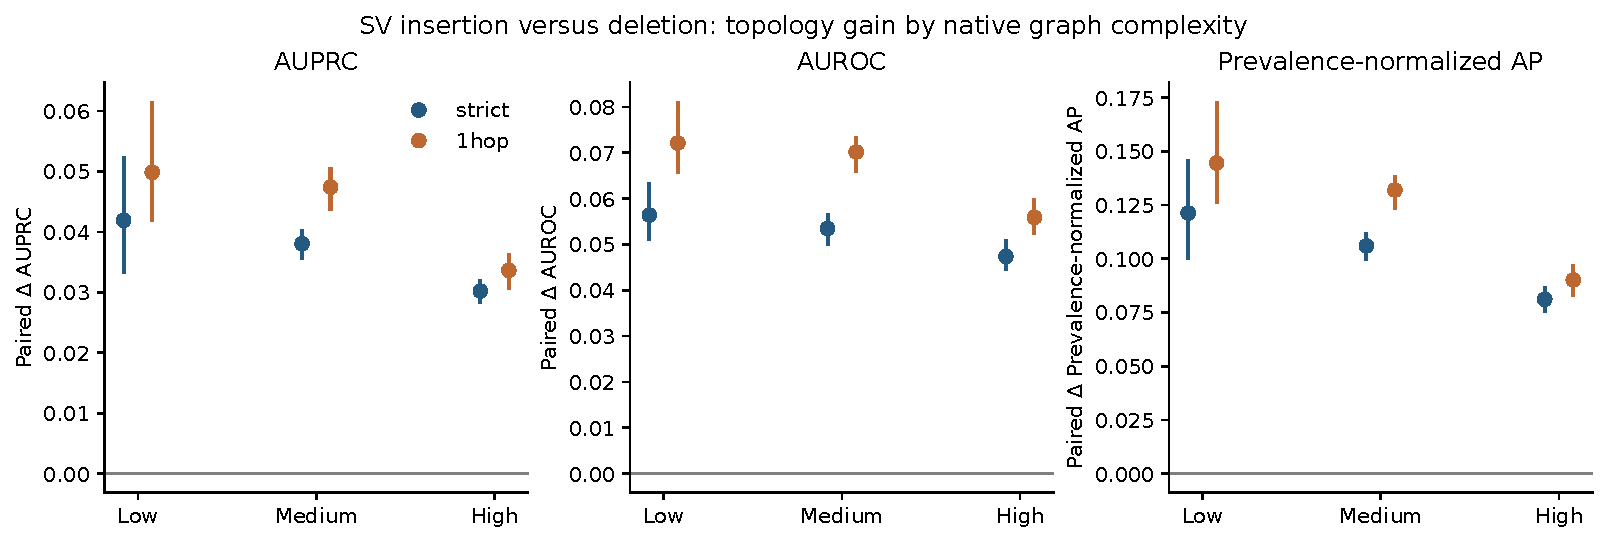
\includegraphics[width=0.95\linewidth]{figures/SuppFig2_sv_complexity.pdf}
\caption{\textbf{Graph contribution to insertion-versus-deletion classification across complexity groups.} Paired gains in AUPRC, AUROC and prevalence-normalized AP on identical held-out examples for $C+S$ and $C+S+T$ within each group. Points and intervals summarize five folds and three runs per context; intervals are pointwise hierarchical bootstrap intervals. Complexity thresholds were fixed independently of model outcomes.}
\label{S-sfig:complexity}
\end{figure}

\subsection{Donors}
Phased carrier assignments were joined to each test event, and gains were computed within the events carried by each donor. After excluding the five donors shared between HPRC and HGSVC (with HG002 and NA24385 treated as one individual\cite{supp__ncbi_hg002}), the 60 remaining donors had mean gains of 0.0367 (\CI 0.0339--0.0395) strict and 0.0430 (0.0393--0.0470) one-hop (Supplementary Fig.~\ref{S-sfig:donor}). Donors share many variants and are not independent replicates. Because the probes were trained on pooled labels from other chromosomes, including those of the same donors, these results describe donor-stratified chromosome transfer rather than generalization to unseen individuals.

\begin{figure}[H]
\centering
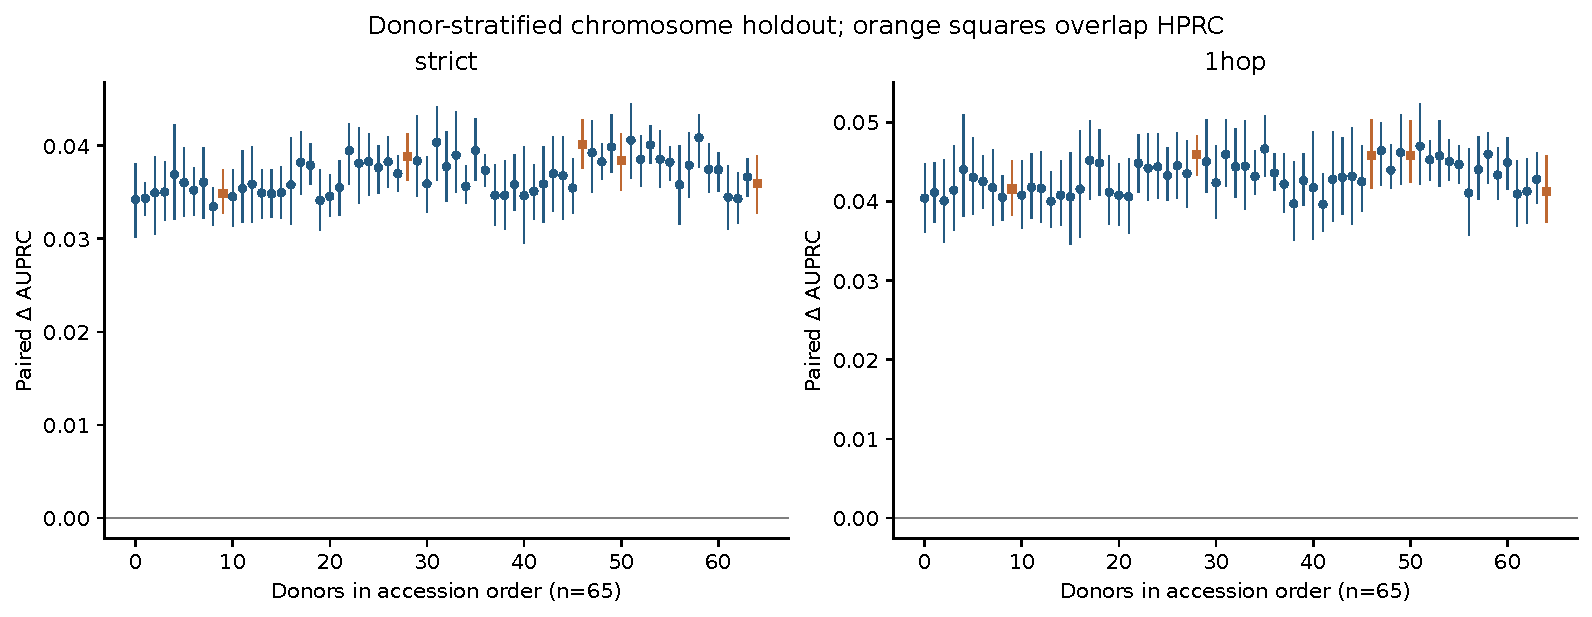
\includegraphics[width=0.95\linewidth]{figures/SuppFig3_donor_stratified_sv.pdf}
\caption{\textbf{Donor-stratified insertion-versus-deletion classification.} Paired graph gains beyond $C+S$ for each HGSVC3 donor, with fold and run bootstrap intervals. Donors are ordered by accession; orange squares mark donors shared with HPRC, including the HG002/NA24385 alias.}
\label{S-sfig:donor}
\end{figure}

%======================================================================
\section{Three-class SV classification}
\label{S-snote:threeclass}

\subsection{Data}
We re-derived event annotations from the source call set while retaining the original event identifiers, verifying insertion and deletion coordinates and allele lengths. The primary-chromosome universe comprises 110,623 insertions, 63,346 deletions and 298 inversions; 2,264 events on non-primary contigs, including two inversions, were excluded. Each event is anchored to the graph segment containing its first affected base. Segment representations for one terminal chrY segment used by 64 events were missing from the original extraction and were generated from the same pretrained encoders, leaving all existing vectors unchanged; no event was dropped. All probe fits in both the natural-frequency and matched analyses converged.

\subsection{Natural-frequency analysis}
Macro AP rose from 0.4070 for $C+S$ to 0.4740 strict and 0.4586 one-hop with $T$ (main Table~\ref{tab:sv-natural}). After $C+S+L+H$, the macro increments were 0.0477 and 0.0150, and the inversion-specific increments were 0.0152 ($-0.0043$ to 0.0365) strict and $-0.0015$ ($-0.0197$ to 0.0117) one-hop. The inversion class is small, and its AP should be judged against a prevalence of 0.0017.

\subsection{Matched sensitivity analysis}
To remove differences in chromosome and length distribution between classes, we sampled 223 events of each type within fixed chromosome and length bins (669 events). This excludes 75 primary-chromosome inversions without matched support, whereas all 298 inversions remain in the natural-frequency analysis. In this matched population, macro AP was 0.4141 for $C+S$ and 0.4738 for $C+S+H$, higher than $C+S+T$ (0.4378 strict, 0.4409 one-hop), and adding $T$ after $H$ was inconclusive (Supplementary Table~\ref{S-stab:svmatched}). Absolute AP should not be compared between the matched and natural-frequency populations, which differ in prevalence and composition. Neither three-class analysis includes an untrained-encoder arm.

\begin{table}[H]
\centering
\caption{\textbf{Macro AP increments from adding $T$ in the matched three-class population.} $P$, exact fold-level sign-flip test; $q$, Benjamini--Hochberg adjustment within the metric.}
\label{S-stab:svmatched}
\footnotesize
\begin{tabular}{@{}llrlrr@{}}
\toprule
Conditioning features & Context & $\Delta_T$ & 95\% CI & $P$ & $q$ \\
\midrule
$C+S$ & Strict & 0.0236 & 0.0158 to 0.0320 & 0.0625 & 0.286 \\
$C+S$ & One-hop & 0.0267 & 0.0041 to 0.0508 & 0.1250 & 0.364 \\
$C+S+H$ & Strict & 0.0025 & $-$0.0052 to 0.0115 & 0.6250 & 0.875 \\
$C+S+H$ & One-hop & $-$0.0019 & $-$0.0118 to 0.0082 & 0.8125 & 0.875 \\
\bottomrule
\end{tabular}
\end{table}

%======================================================================
\section{Sequence-embedding coverage}
\label{S-snote:coverage}

We generated 512-dimensional Nucleotide Transformer embeddings for all 303,425 segments required by the cCRE and SV tasks, in four processing batches with the same model revision. Quality checks confirmed finite values, unique segment identifiers and complete task coverage. Segments longer than the model's input limit (26.3\% of those required) were represented by equal samples from their two ends, up to 6,000 bases, before the tokenizer's maximum-length rule was applied. For such segments the embedding reflects the segment boundaries rather than its full content, which is why the main text interprets the reciprocal sequence contribution for this representation only.

We subsequently extended the embeddings to all 751,237 segments of the graph with the same model and procedure. The 479,477 embeddings used by the reconstruction benchmark were preserved exactly, and 271,760 new embeddings were added, all finite. This extension can provide sequence inputs throughout the graph for future sequence-conditioned models; the analyses reported here, including those in Supplementary Note~\ref{S-snote:objectives}, used the original embeddings.

%======================================================================
\section{EN-TEx datasets and complete results}
\label{S-snote:entex}

\subsection{Datasets}
The AS-prone cCRE dataset contains 5,330,335 informative measurements at 250,722 testable elements, of which 28,092 (11.20\%) are positive. The ENCODE V2 registry annotation ENCFF924IMH matched all active and repressed source accessions, whereas later registry versions left accessions unmatched. The five tissues that met the predefined size rule for the enhancer-state task were thyroid gland, tibial nerve, pancreas, gastroesophageal sphincter and Peyer's patch. The supplied high-confidence SNV file contained only RNA-seq records, so we parsed the 22,310,439 rows of the default accessible call set, retaining 2,391,015 CTCF measurements at 596,650 loci (3.51\% AS) and 3,168,525 H3K27ac measurements at 713,418 loci (2.36\% AS).

\subsection{Results}
All predefined endpoints are shown in Supplementary Table~\ref{S-stab:entex}. The exposure-matched version of the AS-prone cCRE task controls the number of measurement opportunities but targets a different population with higher prevalence, so its absolute AP cannot be compared with the primary task. The prevalence of AS-prone cCREs rises across complexity groups, but that association between complexity and the label does not show that graph representations improve prediction; within-stratum comparisons are required for that conclusion. Intervals are pointwise and unadjusted across the panel.

\begin{table}[H]
\centering
\caption{\textbf{EN-TEx results.} AP for $C+S$ and $C+S+T$ and their paired difference, over five chromosome folds and three runs per context. The enhancer-state task averages five tissues with equal weight. AS, allele-specific; dELS, distal enhancer-like element; ASE, allele-specific expression.}
\label{S-stab:entex}
\footnotesize
\setlength{\tabcolsep}{4pt}
\begin{tabular}{@{}p{0.36\linewidth}lrrrl@{}}
\toprule
Endpoint & Context & $C+S$ & $C+S+T$ & $\Delta_T$ & 95\% CI \\
\midrule
AS-prone cCRE (primary) & Strict & 0.1514 & 0.1516 & 0.00021 & $-$0.00032 to 0.00075 \\
 & One-hop & 0.1514 & 0.1508 & $-$0.00065 & $-$0.00209 to 0.00047 \\
AS-prone cCRE, exposure matched & Strict & 0.5336 & 0.5351 & 0.00148 & 0.00010 to 0.00292 \\
 & One-hop & 0.5336 & 0.5356 & 0.00200 & 0.00084 to 0.00328 \\
AS-prone cCRE, H3K27ac only & Strict & 0.0623 & 0.0629 & 0.00058 & 0.00008 to 0.00107 \\
 & One-hop & 0.0623 & 0.0629 & 0.00061 & $-$0.00053 to 0.00169 \\
AS-prone cCRE, CTCF only & Strict & 0.0781 & 0.0784 & 0.00026 & $-$0.00037 to 0.00095 \\
 & One-hop & 0.0781 & 0.0788 & 0.00073 & 0.00022 to 0.00130 \\
\addlinespace
Active vs repressed dELS (five-tissue mean) & Strict & 0.5699 & 0.5708 & 0.00089 & $-$0.00039 to 0.00233 \\
 & One-hop & 0.5699 & 0.5707 & 0.00080 & $-$0.00153 to 0.00247 \\
\addlinespace
AS SNV, CTCF & Strict & 0.0616 & 0.0630 & 0.00147 & 0.00010 to 0.00355 \\
 & One-hop & 0.0616 & 0.0638 & 0.00225 & 0.00096 to 0.00348 \\
AS SNV, H3K27ac & Strict & 0.0497 & 0.0504 & 0.00069 & $-$0.00057 to 0.00192 \\
 & One-hop & 0.0497 & 0.0530 & 0.00334 & 0.00012 to 0.00796 \\
AS SNV, RNA (ASE) & Strict & 0.0255 & 0.0271 & 0.00157 & $-$0.00008 to 0.00440 \\
 & One-hop & 0.0255 & 0.0270 & 0.00147 & $-$0.00022 to 0.00430 \\
AS SNV, ATAC-seq & Strict & 0.0473 & 0.0470 & $-$0.00031 & $-$0.00071 to 0.00002 \\
 & One-hop & 0.0473 & 0.0476 & 0.00032 & $-$0.00067 to 0.00178 \\
AS SNV, H3K4me3 & Strict & 0.0803 & 0.0847 & 0.00442 & 0.00012 to 0.01061 \\
 & One-hop & 0.0803 & 0.0893 & 0.00900 & 0.00062 to 0.01862 \\
AS SNV, H3K27me3 & Strict & 0.0915 & 0.0949 & 0.00339 & $-$0.00046 to 0.00956 \\
 & One-hop & 0.0915 & 0.0988 & 0.00728 & $-$0.00191 to 0.02133 \\
\bottomrule
\end{tabular}
\end{table}

%======================================================================
\section{External evaluations}
\label{S-snote:external}

\subsection{HG008}
Prospectively refitted probes were evaluated on 69 mapped clonal insertions and deletions in HG008, with no HG008 label used for training. Gains beyond $C+S$ were 0.0325 ($-0.0534$ to 0.1103) strict and 0.0649 ($-0.0667$ to 0.2121) one-hop (Supplementary Table~\ref{S-stab:external}). A single external genome with 69 events cannot establish generalization across individuals. Earlier attempts to re-create the original probes for this genome did not succeed and are not used.

\subsection{TraitGym}
All 14,780 matched variants\cite{supp__benegas2025traitgym} were retained in our five-fold adaptation. Neither the frozen-feature study nor a sensitivity analysis that added published Nucleotide Transformer 2.5B allele scores ($V$) produced a positive topology interval. Before tokenization, the sequence input retained only 22.95\% of tested complex-trait bases and 27.75\% of Mendelian bases, which limits any locus-level sequence representation on this benchmark. In the allele-score sensitivity, the published score alone reached Mendelian AP 0.1604, whereas $C+S+V$ reached 0.1021 compared with 0.1208 for $C+S$, a paired change of $-0.0187$ ($-0.0290$ to $-0.0087$). Replacing the linear probe with a fixed shallow gradient-boosting classifier raised Mendelian $C+S+V$ AP to 0.1711, a gain of 0.0689 (0.0174 to 0.1451). This is a classifier improvement on data that had already been inspected; every topology contrast remained inconclusive or negative.

\subsection{COSIGT call quality}
We summarized 14,838 published sample--locus outcomes at 265 loci\cite{supp__bolognini2026cosigt} into per-locus targets. The training-set median predicted the primary target, the mean quality-value fraction, with mean absolute error 0.0462, compared with 0.0534 for $C+S$ and 0.0527 (strict) and 0.0538 (one-hop) for $C+S+T$. All topology intervals spanned zero. A fallback that used validation error to choose between each fitted model and the median constant reduced error for $C+S+T$ to 0.0479 and 0.0472 but did not establish a topology benefit. These targets describe call quality at released, evaluable sample--locus pairs. They do not measure changes to genotype calls, per-variant concordance or callability across all loci, and they do not address complex or copy-number-variable regions specifically.

\begin{table}[H]
\centering
\caption{\textbf{External endpoints.} Each contrast adds frozen $T$ to $C+S$ over 15 paired fold--run combinations per context. Positive values favour adding $T$; AP gains and reductions in mean absolute error (MAE) have different units.}
\label{S-stab:external}
\footnotesize
\begin{tabular}{@{}lllrl@{}}
\toprule
Endpoint & Context & Metric & Difference & 95\% CI \\
\midrule
HG008 insertions/deletions & Strict & AP gain & 0.0325 & $-$0.0534 to 0.1103 \\
 & One-hop & AP gain & 0.0649 & $-$0.0667 to 0.2121 \\
TraitGym, complex traits & Strict & AP gain & $-$0.0020 & $-$0.0044 to $-$0.0001 \\
 & One-hop & AP gain & $-$0.0010 & $-$0.0036 to 0.0014 \\
TraitGym, Mendelian & Strict & AP gain & $-$0.0051 & $-$0.0176 to 0.0074 \\
 & One-hop & AP gain & 0.0040 & $-$0.0168 to 0.0217 \\
COSIGT call quality & Strict & MAE reduction & 0.0007 & $-$0.0002 to 0.0016 \\
 & One-hop & MAE reduction & $-$0.0005 & $-$0.0016 to 0.0007 \\
\bottomrule
\end{tabular}
\end{table}

%======================================================================
\section{Reconstruction, cross-resource transfer and the degree shortcut}
\label{S-snote:reconstruction}

\subsection{Reconstruction and transfer}
\method recovered hidden connections with region-averaged AP 0.9501 (strict) and 0.9880 (one-hop) on HPRC release~2 and 0.9745 and 0.9868 on HGSVC3 (Supplementary Table~\ref{S-stab:reconstruction}). Transfer without adaptation was direction dependent in the strict context (HPRC to HGSVC 0.5997; HGSVC to HPRC 0.7247) and higher in the one-hop context (0.9408 and 0.8902); transfer between HPRC releases 1.1 and 2 showed the same pattern (Supplementary Fig.~\ref{S-sfig:transfer}). Candidate sets are approximately balanced, so the chance level is about 0.50 (HPRC release~2 prevalence 0.4990 strict and 0.5065 one-hop). Two considerations limit interpretation. All of these scores measure the original objective, which is affected by the degree shortcut described in the main text; and at least five donors are shared between HPRC and HGSVC, so cross-resource rows measure transfer between graph constructions rather than donor-independent generalization.

\begin{table}[H]
\centering
\caption{\textbf{Recovery of hidden connections within and across graph resources and releases.} Region-averaged held-out AP.}
\label{S-stab:reconstruction}
\small
\begin{tabular}{@{}lcc@{}}
\toprule
Training and evaluation & Strict & One-hop \\
\midrule
HPRC release 2, within resource & 0.9501 & 0.9880 \\
HGSVC3, within resource & 0.9745 & 0.9868 \\
Integrated model, HPRC evaluation & 0.9797 & 0.9916 \\
Integrated model, HGSVC evaluation & 0.9786 & 0.9909 \\
Integrated model, combined evaluation & 0.9768 & 0.9894 \\
\midrule
HPRC $\rightarrow$ HGSVC & 0.5997 & 0.9408 \\
HGSVC $\rightarrow$ HPRC & 0.7247 & 0.8902 \\
Integrated $\rightarrow$ HPRC & 0.7007 & 0.8836 \\
HPRC release 1.1 $\rightarrow$ release 2 & 0.7063 & 0.7846 \\
HPRC release 2 $\rightarrow$ release 1.1 & 0.5669 & 0.8838 \\
\bottomrule
\end{tabular}
\end{table}

\begin{figure}[H]
  \centering
  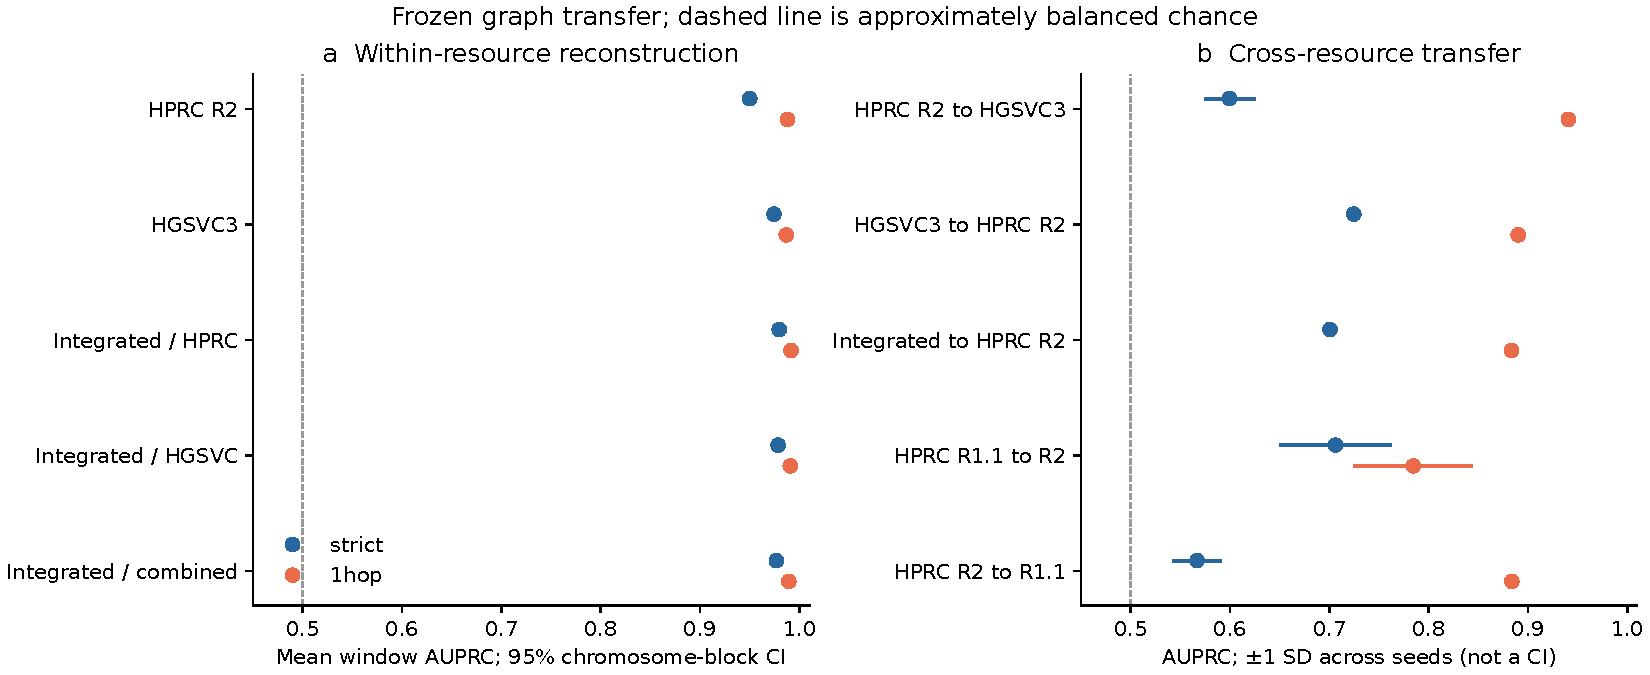
\includegraphics[width=0.95\linewidth]{figures/SuppFig1_reconstruction_transfer.pdf}
  \caption{\textbf{Reconstruction and cross-resource transfer under the original objective.}
  \textbf{a},~Held-out AP for recovering hidden connections within HPRC release~2, HGSVC3 and integrated graphs under strict and one-hop context, with 95\% chromosome-block bootstrap intervals that retain region weighting.
  \textbf{b},~Transfer to a different resource or release without adaptation; whiskers show one standard deviation across three runs and are not confidence intervals.
  All values reflect the original objective, which is affected by the degree shortcut, and cross-resource comparisons involve shared donors.}
  \label{S-sfig:transfer}
\end{figure}

\subsection{Baselines, ablations and capacity}

\begin{figure}[tbp]
  \centering
  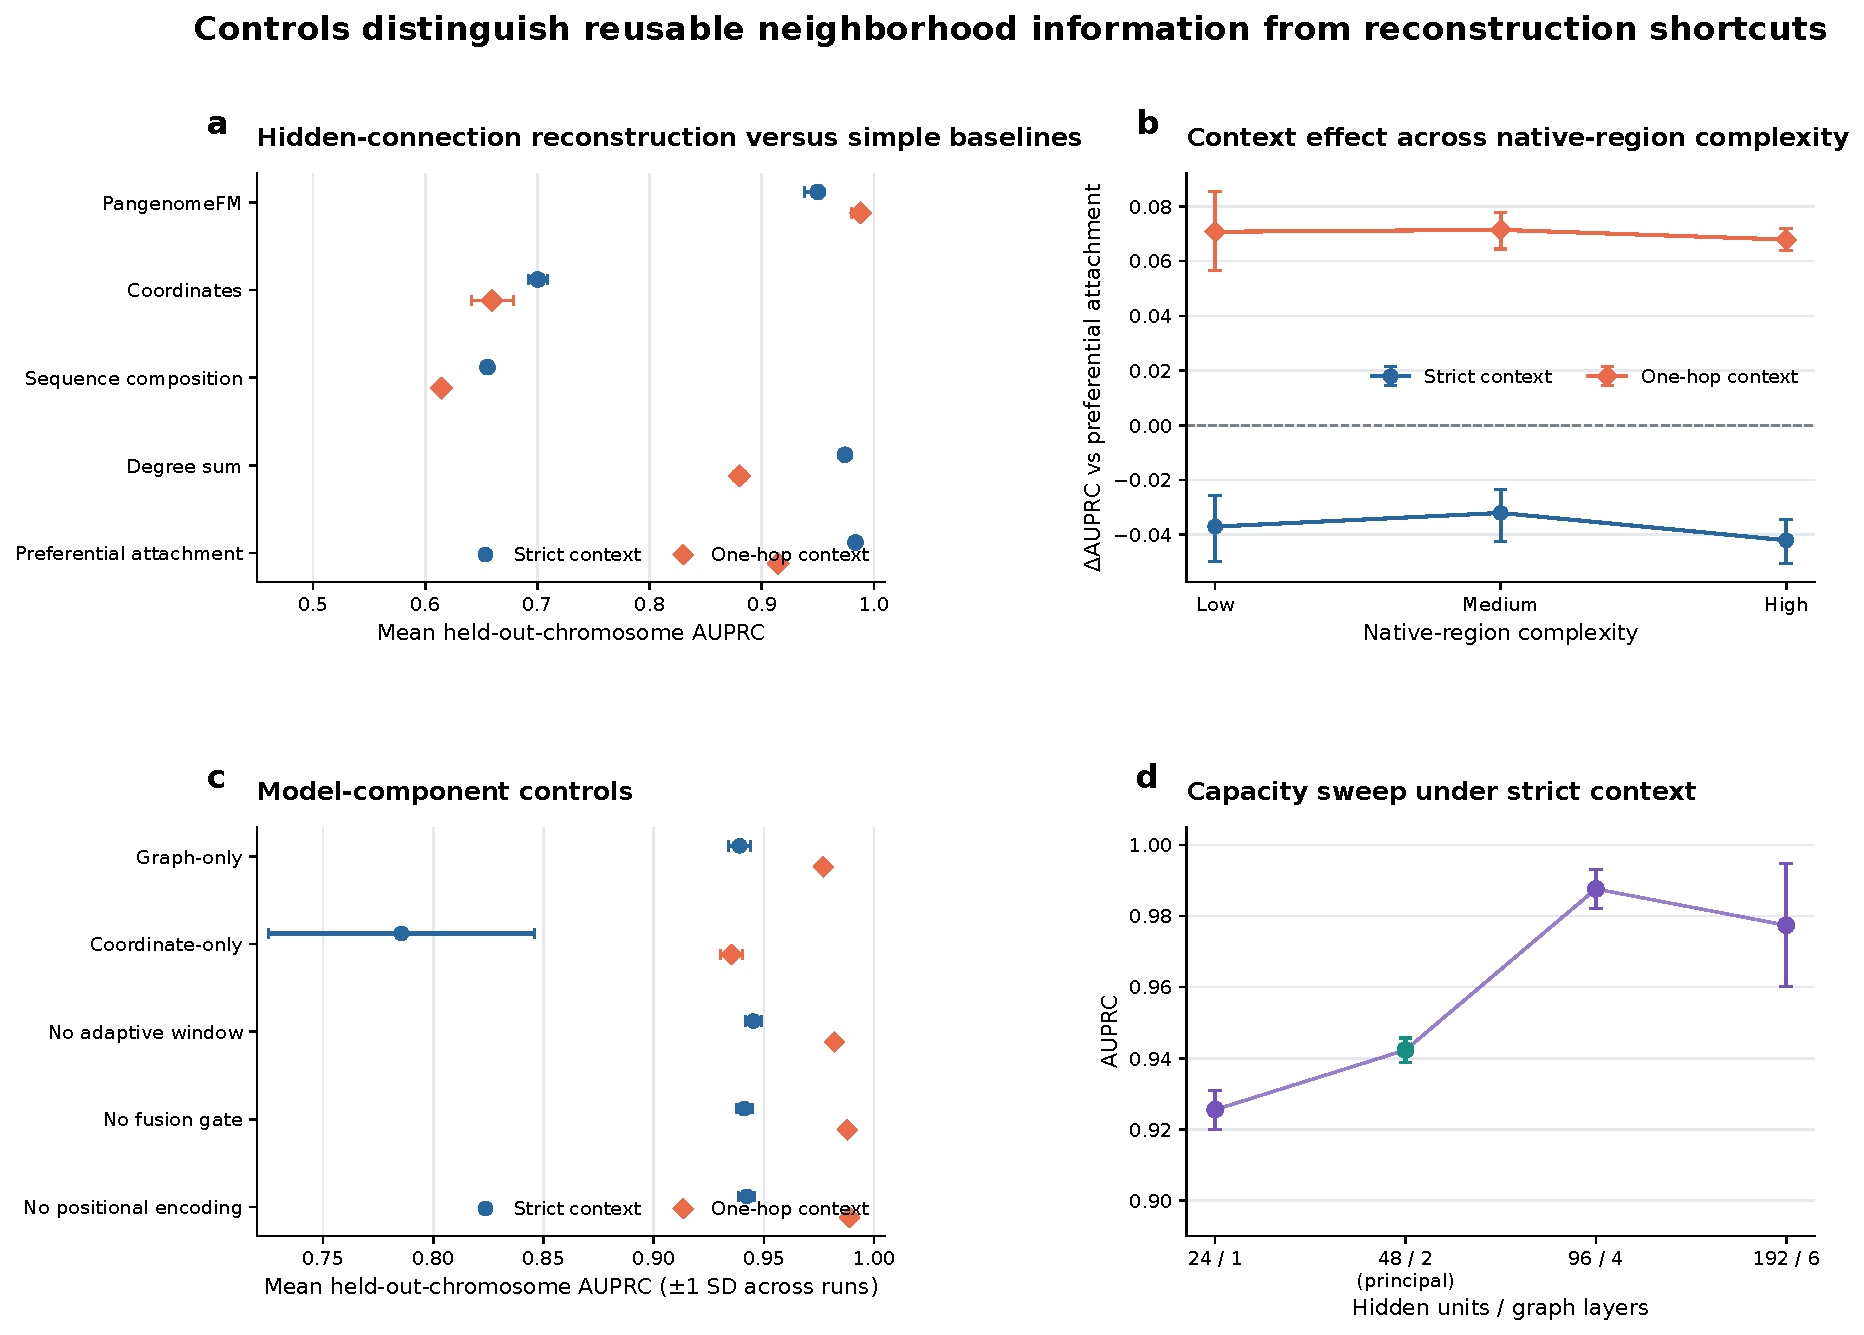
\includegraphics[width=\linewidth]{figures/Fig5_reconstruction_controls.pdf}
  \caption{\textbf{Recovery of hidden connections is dominated by connection counts.}
  \textbf{a},~Held-out-chromosome AP for recovering hidden connections by \method and by simple baselines under strict and one-hop context. The chance level is about 0.50. Preferential attachment and degree sum score candidate pairs by the product and the sum of their endpoints' visible connection counts.
  \textbf{b},~Difference between \method and preferential attachment across native-complexity groups, with 95\% chromosome-block bootstrap intervals.
  \textbf{c},~Component ablations (mean $\pm$ s.d. across runs).
  \textbf{d},~Capacity sweep in the strict context (hidden units / graph layers); the principal configuration is 48/2. AP in \textbf{d} is computed after pooling predictions within each held-out fold and is therefore not directly comparable with the region-averaged AP in \textbf{a}.}
  \label{S-sfig:controls}
\end{figure}
Supplementary Table~\ref{S-stab:baselines} lists the baselines and component ablations shown in main Supplementary Fig.~\ref{S-sfig:controls}. Against preferential attachment, \method had AP differences of $-0.0370$, $-0.0320$ and $-0.0420$ in low-, medium- and high-complexity regions in the strict context, all with intervals excluding zero, and $+0.0707$, $+0.0714$ and $+0.0679$ in the one-hop context. Degree-sum comparisons showed the same reversal. The differences varied far more between contexts than across complexity groups, which does not support an advantage that grows with graph complexity.

Because the degree baselines differ between contexts, we recomputed them from the graph actually visible in each context, including the expanded one-hop graph, after removing each queried connection and its reverse-complement counterpart. The recomputation reproduced all 271,796 reported baseline scores across 1,215 context-specific region sets exactly. The released link tables contain no duplicated reverse-complement links, but the saved predictions do not identify every candidate, so an equivalent traversal of a hidden connection may have remained visible for some candidates during pretraining.

The capacity sweep was non-monotonic (Supplementary Table~\ref{S-stab:capacity}). The 96/4 model reached the highest fold-pooled AP, above the larger 192/6 model. The principal 48/2 model has fold-pooled AP 0.9423 and region-averaged AP 0.9501; these are two summaries of the same predictions, not two models. Given the shortcut, higher reconstruction AP with capacity should not be read as a scaling law for biological transfer.

\begin{table}[H]
\centering
\caption{\textbf{Baselines and component ablations for recovering hidden connections on HPRC release~2.} Mean held-out AP.}
\label{S-stab:baselines}
\small
\begin{tabular}{@{}lcc@{}}
\toprule
Method or ablation & Strict & One-hop \\
\midrule
\method (full model) & 0.9501 & 0.9880 \\
\midrule
Genomic coordinates & 0.7003 & 0.6596 \\
K-mer composition & 0.6555 & 0.6146 \\
Degree sum & 0.9742 & 0.8801 \\
Preferential attachment & 0.9835 & 0.9147 \\
\midrule
Coordinate attention only & 0.7855 & 0.9353 \\
Graph attention only & 0.9390 & 0.9770 \\
Without adaptive window & 0.9452 & 0.9821 \\
Without gate & 0.9411 & 0.9879 \\
Without positional encoding & 0.9423 & 0.9889 \\
\bottomrule
\end{tabular}
\end{table}

\begin{table}[H]
\centering
\caption{\textbf{Capacity sweep in the strict context.} AP after pooling held-out predictions within each fold, a different summary from the region-averaged AP in Supplementary Table~\ref{S-stab:reconstruction}.}
\label{S-stab:capacity}
\small
\begin{tabular}{@{}lccc@{}}
\toprule
Configuration & Hidden dimension & Graph layers & AP \\
\midrule
Small & 24 & 1 & 0.9255 \\
Principal & 48 & 2 & 0.9423 \\
Intermediate & 96 & 4 & 0.9876 \\
Large & 192 & 6 & 0.9774 \\
\bottomrule
\end{tabular}
\end{table}

%======================================================================
\section{Training-window scaling}
\label{S-snote:scaling}

To test whether more unlabelled graph improves the representation, we kept the 52,033-parameter encoder and scorer, the graph, the objective, the folds and the runs fixed and trained on nested, chromosome-balanced subsets containing 12.5\%, 25\%, 50\% and 100\% of training regions. Validation and test candidates were identical across fractions, and the full-data model was retrained under the same conditions rather than taken from earlier results. Realized fractions differ slightly from the nominal values because of rounding within chromosomes and the exclusion of unusable regions.

Fold-pooled reconstruction AP rose from 0.9184 at 12.5\% to 0.9292, 0.9375 and 0.9420 at 25\%, 50\% and 100\% in the strict context, and from 0.9635 to 0.9721, 0.9847 and 0.9900 in the one-hop context (Supplementary Fig.~\ref{S-sfig:scaling}). The 100\%-minus-12.5\% gains were 0.0236 (\CI 0.0216--0.0258) and 0.0265 (0.0253--0.0279). Mean completed epochs ranged from 77.5 to 99.7 across groups, so training compute was not held constant; this is a learning curve under a fixed protocol, not a scaling law.

The corresponding frozen biological evaluation was task dependent. Relative to the 12.5\% model, the 100\% model changed $C+S+T$ AP by $+0.0035$ (0.0031--0.0039) for strict SV classification and $-0.0015$ ($-0.0028$ to $-0.0007$) for one-hop SV classification; cCRE AP improved by 0.0009 (0.0004--0.0015) in the one-hop context and was inconclusive in the strict context ($-0.0003$; $-0.0007$ to 0.0000), and intervals for CTCF allele-specific SNVs included zero. More data improved the pretraining task without consistently improving biological prediction, as expected if the objective rewards the degree cue.

\begin{figure}[H]
\centering
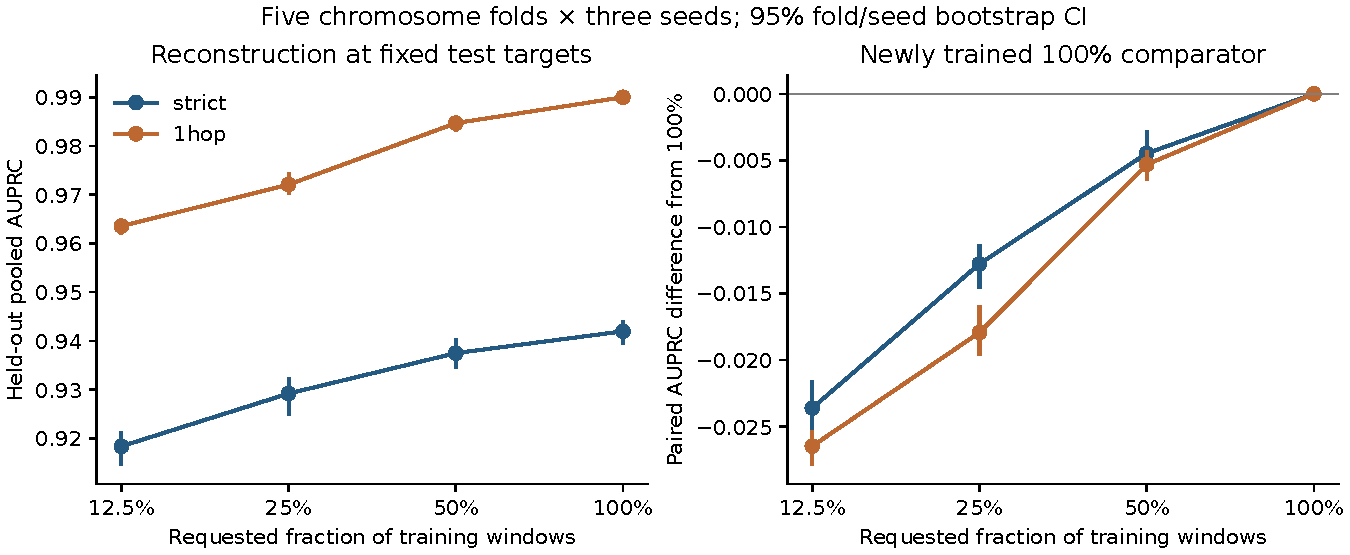
\includegraphics[width=0.9\linewidth]{figures/SuppFig4_training_window_scaling.pdf}
\caption{\textbf{Reconstruction improves with more unlabelled training regions.} Left, fold-pooled held-out AP across five folds and three runs. Right, paired differences from the full-data model on identical test candidates, with 95\% hierarchical bootstrap intervals. Lines connect measured settings; no scaling law is fitted. Model size is fixed, but training compute varies with the number of regions and early stopping.}
\label{S-sfig:scaling}
\end{figure}

%======================================================================
\section{Development of shortcut-resistant objectives}
\label{S-snote:objectives}

\subsection{Rationale}
Under the original objective, every positive endpoint loses a visible connection when the query is hidden, whereas the endpoints of matched negatives need not lose any. We therefore developed two objectives in which this cue is absent by construction (Methods): junction re-pairing, in which positives and negatives are alternative pairings of the same dangling ends, and masked sequence-feature reconstruction, in which connectivity is not a prediction target. Both were developed on fold~A, using its training chromosomes for pretraining and its validation chromosomes (chr2, chr7, chr12, chr17 and chr22) for selection. These chromosomes are the test set of fold~B, which is therefore reported separately in the ongoing chromosome-level replication.

\subsection{Junction re-pairing}
On the development candidates (2,050 pairs in 104 regions, positive fraction 0.50), geometry and degree cues alone were uninformative: endpoint geometry scored 0.5000, visible connection counts 0.5070 and both together 0.5068 (Supplementary Fig.~\ref{S-sfig:objectives}a). Per-segment inputs that include sequence embeddings reached 0.7097 with logistic regression and 0.7340 with gradient boosting, showing that segment content carries some information about which ends belong together. In this configuration, encoders passing messages only along incoming connections remained near chance (trained 0.5007 versus untrained 0.5028 with the multilayer scorer), whereas bidirectional encoders achieved higher AP (0.7897 versus 0.6257; with a linear scorer, 0.7400 versus 0.5448). Adding sequence embeddings to the segment inputs gave 0.8407 and 0.8700 for the two scorers, against 0.6794 and 0.6547 for untrained counterparts and 0.7340 for gradient boosting without the graph (Supplementary Fig.~\ref{S-sfig:objectives}b). These are single-run results on the partition used to choose among designs, and no confidence intervals are attached. Initial-parameter equivalence is verified for the sequence-conditioned pairs but cannot be verified from the older topology-only checkpoints. The latter therefore remain architecture-matched controls with an initialization-provenance limitation. Under the same matching constraints the strict context retained only 12 eligible regions across all chromosomes, too few for training and validation, so development used the one-hop context only.

Frozen representations from the junction-trained encoder were combined with the original representations and evaluated on the biological tasks under a three-run development criterion, which required the combination to exceed every matched combination containing untrained components after $C+S+H$, and not to fall materially below the better single representation, for both tasks. The criterion was met in one of three runs; the other two failed for cCRE and for SV, respectively. This encoder was therefore not advanced to chromosome-level replication.

\begin{figure}[H]
\centering
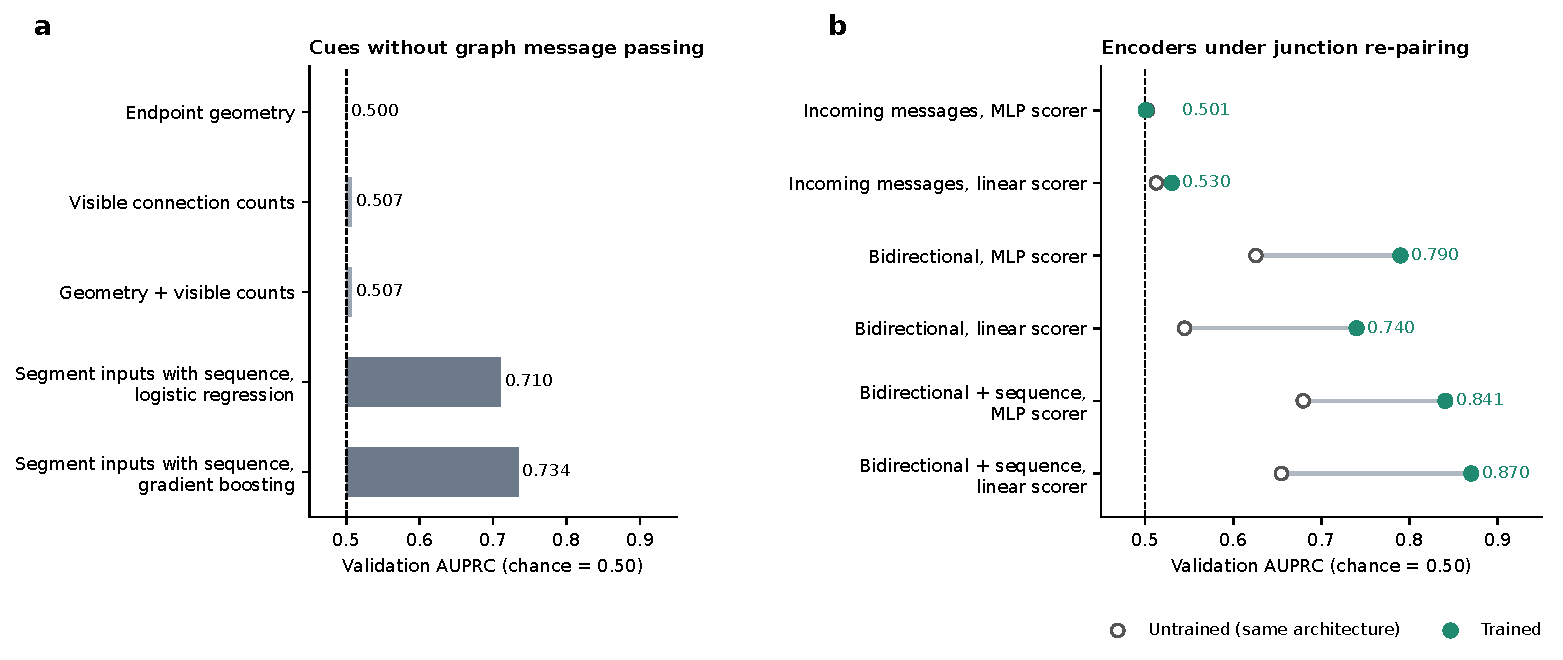
\includegraphics[width=\linewidth]{figures/SuppFig5_objective_development.pdf}
\caption{\textbf{Bidirectional messages improve junction re-pairing in the development comparison.} Development results on fold-A validation chromosomes in the one-hop context (2,050 candidate pairs in 104 regions; chance AUPRC 0.50).
\textbf{a},~Cues available without graph message passing: endpoint geometry and visible connection counts score at chance; per-segment inputs, including sequence embeddings, carry some information.
\textbf{b},~Trained encoders (filled) and untrained encoders of the same architecture (open) for incoming-only and bidirectional message passing, with multilayer or linear pair scorers, without or with sequence embeddings as segment inputs. Single runs; no confidence intervals.}
\label{S-sfig:objectives}
\end{figure}

\subsection{Masked sequence-feature reconstruction}
Twelve pretraining runs (four arms by three runs) and the corresponding frozen probes were completed, and all probes converged. On fold-A validation chromosomes, the trained-minus-untrained AP difference after $C+S+H$ averaged 0.0056 for insertion-versus-deletion classification and 0.0018 for cCREs and was positive in every run (Supplementary Table~\ref{S-stab:development}). Full encoders also exceeded coordinate-only encoders in every run, by 0.0061 and 0.0024 on average; because the coordinate-only ablation also removes capacity, this is not an isolated estimate of the effect of message passing. F1 and balanced accuracy were not uniformly better in every run. Against the junction-trained encoder of the same width, the masked-feature encoder had a mean AP advantage after $C+S+H$ of 0.0019 for insertion-versus-deletion classification and 0.0001 for cCREs, with training budgets that differed (20 versus 10 epochs).

These three runs share one development block and do not provide an estimate of chromosome-level uncertainty. The chromosome-level replication on all five folds, with fold~B reported separately, and a matched comparison with the original encoder are in progress; no partial results enter this paper. Development success therefore does not establish superiority over the original encoder, external transfer or a general-purpose foundation model.

\begin{table}[H]
\centering
\caption{\textbf{Masked sequence-feature encoder ($E$): development controls.} AP after $C+S+H$ on fold-A validation chromosomes for each of three runs. Trained--untrained is the full trained encoder minus its untrained counterpart; full--coordinate is the full trained encoder minus the coordinate-only trained encoder, which also has less capacity. Runs 1--3 correspond to run identifiers 42, 314159 and 20260806.}
\label{S-stab:development}
\footnotesize
\setlength{\tabcolsep}{5pt}
\begin{tabular}{@{}llrrrr@{}}
\toprule
Run & Task & Trained & Untrained & Trained $-$ untrained & Full $-$ coordinate \\
\midrule
1 & Insertion vs deletion & 0.9064 & 0.9009 & 0.0055 & 0.0045 \\
1 & cCRE & 0.9208 & 0.9194 & 0.0014 & 0.0027 \\
2 & Insertion vs deletion & 0.9072 & 0.9007 & 0.0065 & 0.0076 \\
2 & cCRE & 0.9207 & 0.9185 & 0.0022 & 0.0020 \\
3 & Insertion vs deletion & 0.9071 & 0.9023 & 0.0049 & 0.0063 \\
3 & cCRE & 0.9208 & 0.9188 & 0.0019 & 0.0024 \\
\bottomrule
\end{tabular}
\end{table}

%======================================================================
\section{Matched overlap with QTL and GWAS signals}
\label{S-snote:overlap}

As an exploratory test of whether regions prioritized by the model coincide with genetic association signals, we selected the highest-scoring 10\% of 5-Mb regions within each chromosome and matched each to five control regions (Supplementary Methods). None of the evaluated signal sets showed greater overlap with prioritized regions than with matched controls (Supplementary Table~\ref{S-stab:overlap}). The all-trait GWAS set overlapped every prioritized and control region, so that comparison is saturated. This analysis measures broad regional overlap only and provides no evidence about colocalization, fine mapping, causal association or phenotype prediction.

\begin{table}[H]
\centering
\caption{\textbf{Overlap of model-prioritized regions with QTL and GWAS signals.} $P_{>}$ is the one-sided permutation probability of greater overlap in prioritized regions than in matched controls.}
\label{S-stab:overlap}
\small
\begin{tabular}{@{}lrrrlr@{}}
\toprule
Signal set & Sets & Case hit & Control hit & Risk difference (95\% CI) & $P_{>}$ \\
\midrule
eQTL, chr8 & 45 & 0.0444 & 0.0400 & 0.0044 (0.0000 to 0.0133) & 0.832 \\
sQTL, chr8 & 45 & 0.0222 & 0.0400 & $-0.0178$ ($-0.0533$ to 0.0000) & 1.000 \\
GWAS, all traits & 45 & 1.0000 & 1.0000 & 0.0000 (0.0000 to 0.0000) & 1.000 \\
GWAS, Parkinson's disease & 45 & 0.1333 & 0.2178 & $-0.0844$ ($-0.1867$ to 0.0223) & 0.942 \\
\bottomrule
\end{tabular}
\end{table}

%======================================================================
\section*{Supplementary Methods}
\addcontentsline{toc}{section}{Supplementary Methods}

\subsection{Chromosome partitions}
Every primary chromosome appears in exactly one test block across the five-fold rotation (Supplementary Table~\ref{S-stab:folds}). All chromosomes outside the test and validation blocks of a fold form its training set.

\begin{table}[H]
\centering
\caption{\textbf{Rotating chromosome partitions.}}
\label{S-stab:folds}
\small
\begin{tabularx}{\linewidth}{@{}lXX@{}}
\toprule
Fold & Test chromosomes & Validation chromosomes \\
\midrule
A & chr1, chr6, chr11, chr16, chr21 & chr2, chr7, chr12, chr17, chr22 \\
B & chr2, chr7, chr12, chr17, chr22 & chr3, chr8, chr13, chr18, chrX \\
C & chr3, chr8, chr13, chr18, chrX & chr4, chr9, chr14, chr19, chrY \\
D & chr4, chr9, chr14, chr19, chrY & chr5, chr10, chr15, chr20 \\
E & chr5, chr10, chr15, chr20 & chr1, chr6, chr11, chr16, chr21 \\
\bottomrule
\end{tabularx}
\end{table}

\subsection{Haplotype path extraction}
Haplotype paths were extracted from GBZ graph files\cite{supp__siren2022gbz} and linked to full-resolution segment indexes. Observed traversals were sampled within 5-Mb windows and checked for missing segment handles. No path-specific unobserved connections were generated.

\subsection{TraitGym adaptation}
We preserved TraitGym's matched groups (one positive and nine controls), alleles and chromosome-X examples, and assigned variants to our five chromosome folds rather than the official leave-one-chromosome-out protocol, so results are not comparable with the benchmark leaderboard. The published allele scores $V$ comprise signed and absolute masked-allele log-likelihood ratios from Nucleotide Transformer 2.5B, joined by verified row order and variant identity. The classifier sensitivity analysis selected linear regularization from six values on validation data, used a fixed 150-iteration shallow histogram gradient-boosting classifier, and evaluated four validation-selected late-fusion combinations.

\subsection{COSIGT targets}
The primary continuous target was the mean quality-value fraction at each locus; the mean predicted quality value was a secondary target. Seven ridge penalties were compared on validation mean absolute error, with stronger regularization breaking exact ties. The training-median constant, locus length and $H$ were retained as explicit references. The publisher's reference panel excludes its test donors, but donor overlap with the graph used to train \method remains possible.

\subsection{EN-TEx multiplicity}
For allele-specific SNV tasks, all occurrences of a genomic position were assigned to the same chromosome fold, measurement multiplicities were retained as sample weights and every occurrence of a locus received the same prediction. This design tests locus-level susceptibility rather than the direction of imbalance in a given donor.

\subsection{Matched overlap analysis}
Regions were ranked by model prioritization within each chromosome. Each of the top 10\% of regions was matched to five controls on region length, GC content, Umap/Bismap mappability\cite{supp__karimzadeh2018umap}, graph complexity, HPRC variant density and distance to the nearest GENCODE v50 gene\cite{supp__frankish2023gencode}. Signal sets comprised chromosome-8 eQTL and sQTL positions\cite{supp__lappalainen2013transcriptome}, all-trait GWAS Catalog positions and positions filtered for Parkinson's disease\cite{supp__sollis2023gwas}. The QTL analysis was a prespecified chromosome-8 pilot: only the chromosome-8 summary files were retrieved, after checking download size and local storage, and the chromosome was not selected on the basis of enrichment. Inference used 10,000 one-sided matched permutations and 2,000 bootstrap replicates for intervals.

\subsection{Recorded settings}
For every principal analysis we recorded the model configuration, pretrained model version, held-out chromosomes, run identifier, graph context, excluded candidate pairs, predictions and metrics, and summaries required every prescribed fold--run combination to be complete.

%======================================================================
\section*{Consortium authors}
\addcontentsline{toc}{section}{Consortium authors}
\noindent\textbf{Human Pangenome Reference Consortium.} \authorinput{member list and affiliations to be provided by the consortium}

\noindent\textbf{Human Genome Structural Variation Consortium.} \authorinput{member list and affiliations to be provided by the consortium}

\FloatBarrier
\begingroup
\small
\renewcommand{\refname}{Supplementary references}
\begin{thebibliography}{11}
\providecommand{\natexlab}[1]{#1}
\providecommand{\url}[1]{\texttt{#1}}
\expandafter\ifx\csname urlstyle\endcsname\relax
  \providecommand{\doi}[1]{doi: #1}\else
  \providecommand{\doi}{doi: \begingroup \urlstyle{rm}\Url}\fi

\bibitem[Dalla-Torre et~al.(2025)Dalla-Torre, Gonzalez, Mendoza-Revilla,
  Carranza, Grzywaczewski, Oteri, Dallago, Trop, de~Almeida, Sirelkhatim,
  et~al.]{supp__dalla2025nucleotide}
Hugo Dalla-Torre, Liam Gonzalez, Javier Mendoza-Revilla, Nicolas~Lopez
  Carranza, Adam~Henryk Grzywaczewski, Francesco Oteri, Christian Dallago, Evan
  Trop, Bernardo~P. de~Almeida, Hassan Sirelkhatim, et~al.
\newblock Nucleotide transformer: building and evaluating robust foundation
  models for human genomics.
\newblock \emph{Nature Methods}, 22\penalty0 (2):\penalty0 287--297, 2025.
\newblock \doi{10.1038/s41592-024-02523-z}.

\bibitem[Liao et~al.(2023)Liao, Asri, Ebler, Doerr, Haukness, Hickey, Lu,
  Lucas, Monlong, Abel, et~al.]{supp__hprc2023draft}
Wen-Wei Liao, Mobin Asri, Jana Ebler, Daniel Doerr, Marina Haukness, Glenn
  Hickey, Shuangjia Lu, Julian~K. Lucas, Jean Monlong, Haley~J. Abel, et~al.
\newblock A draft human pangenome reference.
\newblock \emph{Nature}, 617\penalty0 (7960):\penalty0 312--324, 2023.
\newblock \doi{10.1038/s41586-023-05896-x}.

\bibitem[Logsdon et~al.(2025)]{supp__hgsvc32025}
Glennis~A. Logsdon et~al.
\newblock Complex genetic variation in nearly complete human genomes.
\newblock \emph{Nature}, 644:\penalty0 430--441, 2025.

\bibitem[{National Center for Biotechnology
  Information}(2026)]{supp__ncbi_hg002}
{National Center for Biotechnology Information}.
\newblock {NIST HG002 NA24385: BioSample SAMN03283347}.
\newblock \url{https://www.ncbi.nlm.nih.gov/biosample/SAMN03283347/}, 2026.
\newblock Database record accessed 24 September 2026.

\bibitem[Benegas et~al.(2025)Benegas, Eraslan, and
  Song]{supp__benegas2025traitgym}
Gonzalo Benegas, G{\"o}kcen Eraslan, and Yun~S. Song.
\newblock Benchmarking {DNA} sequence models for causal regulatory variant
  prediction in human genetics.
\newblock \emph{bioRxiv}, 2025.
\newblock \doi{10.1101/2025.02.11.637758}.

\bibitem[Bolognini et~al.(2026)]{supp__bolognini2026cosigt}
Davide Bolognini et~al.
\newblock {COSIGT}: population-scalable genotyping of complex loci from
  low-coverage sequencing data using pangenome graphs.
\newblock \emph{Genome Biology}, 27:\penalty0 286, 2026.
\newblock \doi{10.1186/s13059-026-04242-4}.

\bibitem[Sir{\'e}n and Paten(2022)]{supp__siren2022gbz}
Jouni Sir{\'e}n and Benedict Paten.
\newblock {GBZ} file format for pangenome graphs.
\newblock \emph{Bioinformatics}, 38\penalty0 (22):\penalty0 5012--5018, 2022.
\newblock \doi{10.1093/bioinformatics/btac656}.

\bibitem[Karimzadeh et~al.(2018)Karimzadeh, Ernst, Kundaje, and
  Hoffman]{supp__karimzadeh2018umap}
Mehran Karimzadeh, Carl Ernst, Anshul Kundaje, and Michael~M. Hoffman.
\newblock {Umap} and {Bismap}: quantifying genome and methylome mappability.
\newblock \emph{Bioinformatics}, 34\penalty0 (13):\penalty0 i716--i725, 2018.
\newblock \doi{10.1093/bioinformatics/bty617}.

\bibitem[Frankish et~al.(2023)]{supp__frankish2023gencode}
Adam Frankish et~al.
\newblock {GENCODE}: reference annotation for the human and mouse genomes in
  2023.
\newblock \emph{Nucleic Acids Research}, 51\penalty0 (D1):\penalty0 D942--D949,
  2023.
\newblock \doi{10.1093/nar/gkac1071}.

\bibitem[Lappalainen et~al.(2013)Lappalainen, Sammeth, Friedl{\"a}nder,
  et~al.]{supp__lappalainen2013transcriptome}
Tuuli Lappalainen, Michael Sammeth, Marc~R. Friedl{\"a}nder, et~al.
\newblock Transcriptome and genome sequencing uncovers functional variation in
  humans.
\newblock \emph{Nature}, 501:\penalty0 506--511, 2013.
\newblock \doi{10.1038/nature12531}.

\bibitem[Sollis et~al.(2023)Sollis, Mosaku, Abid, Buniello, Cerezo, Gil, Groza,
  G{\"u}nes, Hall, Hayhurst, et~al.]{supp__sollis2023gwas}
Elliott Sollis, Abiodun Mosaku, Anum Abid, Annalisa Buniello, Maria Cerezo,
  Laura Gil, Tudor Groza, Oya G{\"u}nes, Peggy Hall, James Hayhurst, et~al.
\newblock The {NHGRI-EBI GWAS Catalog}: knowledgebase and deposition resource.
\newblock \emph{Nucleic Acids Research}, 51\penalty0 (D1):\penalty0 D977--D985,
  2023.
\newblock \doi{10.1093/nar/gkac1010}.

\end{thebibliography}

\endgroup


\end{document}

% BEGIN PRESERVED PROFESSOR COMMENTS
% Long Note: Original attachment comments are preserved verbatim below, including resolved and superseded requests.
% Long Note: Original line anchors identify the supplied attachment; these comments do not replace the current manuscript.
% Long Note: Dispositions and new editorial responses remain beside the relevant current text and in the comment-response audit.

% Long Note: Original attachment line 3.
% Prevent pdflatex object-stream overflow with complex vector figures.
% Long Note: Done [T01]. Original compression workaround retained with an engine guard;
% native multiproject compilation is checked separately.

% Long Note: Original attachment line 27.
% Uncomment if line numbers are required.

% Long Note: Original attachment line 28.
% \usepackage[mathlines]{lineno}\linenumbers
% Long Note: Done [T02]. Optional line-numbering switch retained, not activated without a
% submission requirement.

% Long Note: Original attachment line 44.
% \titleformat{\section}{\large\bfseries}{\thesection.}{0.6em}{}

% Long Note: Original attachment line 45.
% \titleformat{\subsection}{\normalsize\bfseries}{\thesubsection.}{0.6em}{}
% Long Note: Done [T03]. Commented formatting alternatives retained; active headings are
% unnumbered.

% Long Note: Original attachment line 58.
%
% Long Note: Done [T04]. Macro whitespace-control comment retained.

% Long Note: Original attachment line 71.
% Nature Machine Intelligence
% Long Note: Done [T05]. Venue/style note retained; no acceptance claim is inferred.

% Long Note: Original attachment line 75.
% Pangenome Foundation Model capture
% Long Note: Done [T06]. Title scopes the contribution to topology-native representation
% learning.

% Long Note: Original attachment line 76.
% Need to add HGSVC and HPRC to the author list

% Long Note: Original attachment line 82.
% HGSVC, HPRC,
% Long Note: Author input needed [A01]. Exact approved consortium author wording, membership
% and approval are unavailable.

% Long Note: Original attachment line 101.
% NEW STRUCTURES

% Long Note: Original attachment line 103.
% Title

% Long Note: Original attachment line 104.
% Abstract

% Long Note: Original attachment line 106.
% Introduction

% Long Note: Original attachment line 108.
% Results

% Long Note: Original attachment line 109.
%   1. Graph-native representations add complementary information to regulatory-element prediction

% Long Note: Original attachment line 110.
%   2. Graph-native representations contribute strongly to structural-variant breakpoint classification

% Long Note: Original attachment line 111.
%   3. Frozen graph representations generalize across chromosomes and transfer across pangenome resources

% Long Note: Original attachment line 112.
%   4. Neighborhood context distinguishes learned graph representations from degree-based shortcuts

% Long Note: Original attachment line 114.
% Discussion

% Long Note: Original attachment line 116.
% Methods

% Long Note: Original attachment line 117.
%   Pangenome resources and graph preparation

% Long Note: Original attachment line 118.
%   Masked graph-connection pretraining

% Long Note: Original attachment line 119.
%   PangenomeFM architecture

% Long Note: Original attachment line 120.
%   Strict and one-hop graph context

% Long Note: Original attachment line 121.
%   Chromosome-held-out evaluation

% Long Note: Original attachment line 122.
%   Cross-resource and cross-release transfer

% Long Note: Original attachment line 123.
%   Sequence embeddings and downstream classifiers

% Long Note: Original attachment line 124.
%   Baselines, ablations and capacity

% Long Note: Original attachment line 125.
%   Statistical analysis

% Long Note: Original attachment line 126.
%   Exploratory path/QTL/GWAS analyses

% Long Note: Original attachment line 128.
% Data availability

% Long Note: Original attachment line 129.
% Code availability

% Long Note: Original attachment line 130.
% Acknowledgements

% Long Note: Original attachment line 131.
% Funding

% Long Note: Original attachment line 132.
% Author contributions

% Long Note: Original attachment line 133.
% References

% Long Note: Original attachment line 135.
% Supplementary Information
% Long Note: Done [T07]. Historical outline retained as comments; the revised method-led
% structure supersedes its ordering.

% Long Note: Original attachment line 146.
% Structure: biological representation problem --> graph-native idea --> cCRE --> SV --> generalization --> control --> scoped conclusion
% Long Note: Done [T08]. Abstract revised around the representation problem, design, evidence
% and attribution limit.

% Long Note: Original attachment line 153.
% Long and Tomoya, here are what I think about the layout of the introduction: representation of DNA sequences and human genomes (linear->graph - capturing diversity, complex variations and regions), existing DNA foundation models and their applications (this can be swapped to the beginning of this session), the need of non-linear/graph representation of genomes and foundation models  to capture information in graph genomes or pangnomes, previous efforts of building pangenome foundation models and what they lack of, -> introduce pangenomeFM, improvement over previous work, applications of using pangenomeFM for downstream tasks.
% Long Note: Done [S01]. Introduction progression implemented; R01.
% Long Note: Done [R01]. Introduction follows the six-paragraph representation-to-method
% progression; see sec:intro.

% Long Note: Original attachment line 157.
% Long, the following paper should be cited (add other related papers if any) to stress the importance of using graph genomes for functional genomics analysis

% Long Note: Original attachment line 158.
% https://www.nature.com/articles/s41467-026-73663-3
% Long Note: Done [S02]. Requested functional-genomics citation verified; R02.
% Long Note: Done [R02]. Macias-Velasco et al. is cited with DOI 10.1038/s41467-026-73663-3;
% its genome/pipeline scope is stated accurately.

% Long Note: Original attachment line 161.
% [LONG NOTE]

% Long Note: Original attachment line 162.
% Para 1: linear to graph: what linear has, what it loses, and why graph could enable the diversity

% Long Note: Original attachment line 163.
% Para 2: why the representation matters in biology

% Long Note: Original attachment line 164.
% para 3: talks about the DNA foundation models (DNABERT,etc.)

% Long Note: Original attachment line 165.
% para 4: talks about pangenome topology features which sequence tokens do not present/have

% Long Note: Original attachment line 166.
% para 5: previous work & gaps (DeepGene, PangenomeX, etc.)

% Long Note: Original attachment line 167.
% para 6: introduce PangenomeFM + evidence/result (main generalization, etc.)
% Long Note: Done [S03]. Six-paragraph outline implemented in sec:intro.

% Long Note: Original attachment line 172.
% Intro should start with the representation of human genomes, genetic variation should be mentioned later
% Long Note: Done [S04]. Representation-first opening retained; R03.
% Long Note: Done [R03]. The Introduction opens with human-genome representation and
% coordinate systems before discussing variation.

% Long Note: Original attachment line 183.
% Long, the layout looks more like a CS paper, we need to change it to the format of Nature Machine Intelligence or Nature Methods (check some recent papers in those journals and follow their layout)
% Long Note: Done [S05]. NMI examples reviewed and structure revised; R04.
% Long Note: Done [R04]. All four supplied NMI examples informed the method-led structure;
% four main figures and two main tables retain key controls.

% Long Note: Original attachment line 187.
% Long, this figure should be cited in Introduction, where you can merge the current related work and background into Introduction
% Long Note: Done [S06]. Paradigm figure cited in integrated Introduction; R05.
% Long Note: Done [R05]. The Introduction integrates background/prior work and cites
% fig:paradigms; no separate Related Work section is needed.

% Long Note: Original attachment line 190.
% TODO(figure): redesign with keyword-only labels. End each paradigm at

% Long Note: Original attachment line 191.
% its learned output; explain downstream reuse in the caption rather than a

% Long Note: Original attachment line 192.
% PangenomeFM-only output column.
% Long Note: Done [T09]. Parallel output figure redesigned and verified; R06.
% Long Note: Done [R06]. The redesigned keyword-led paradigm figure ends every row at its
% learned representation; reuse is explained in the caption.

% Long Note: Original attachment line 264.
% Long, add results on predicting cCREs and ENCODE data?

% Long Note: Original attachment line 265.
% add citation of this paper 

% Long Note: Original attachment line 266.
% https://www.nature.com/articles/s41467-026-73663-3
% Long Note: Done [S07]. cCRE/ENCODE result and requested citation retained; R07/R02.

% Long Note: Original attachment line 268.
% cCRE is now the first standalone Result. The existing binary cCRE

% Long Note: Original attachment line 269.
% result is included below. TODO(new analysis): if ENCODE class labels are cleanly

% Long Note: Original attachment line 270.
% recoverable, add PLS/pELS/dELS/CTCF-only stratification and/or topology gain by

% Long Note: Original attachment line 271.
% local graph/variant complexity. Do not assume which class benefits most.
% Long Note: Done [R07]. Binary cCRE, PLS/pELS/dELS/CTCF-only and fixed complexity strata are
% reported in sec:ccre-result. The old first-Result placement is superseded by the
% method-first order.

% Long Note: Original attachment line 282.
% TODO(new analysis): add cCRE class / complexity stratification here if completed.

% Long Note: Original attachment line 283.
% Recommended tests: PLS, pELS, dELS, CTCF-only; and/or low/medium/high local

% Long Note: Original attachment line 284.
% graph complexity using thresholds fixed independently of model performance.
% Long Note: Done [S08]. Four subclasses and fixed complexity strata reported; R07.

% Long Note: Original attachment line 285.
% Optional biological vignette: one transparently selected locus with graph,

% Long Note: Original attachment line 286.
% annotation track, and predictions; avoid selecting solely by maximal gain.
% Long Note: Optional, not done [S09]. No selected-locus vignette is claimed; it needs
% verified tracks, predictions and a predeclared selection rule.

% Long Note: Original attachment line 320.
% Keep this table:

% Long Note: Original attachment line 321.
% For final NMI submission, consider moving the table to Supplementary once the

% Long Note: Original attachment line 322.
% standalone biological figures carry these values clearly.
% Long Note: Done [T10]. Primary numerical table preserved in Supplement; main biological
% figures retain its outcomes.

% Long Note: Original attachment line 343.
% Is it possible to improve SV genotyping (especially in complex and copy number variant regions)?
% Long Note: Evidence open [M01]. Genotyping assessment answered, but improved calls are not
% established; R08.
% Long Note: Evidence open [R08]. The genotyping question is answered by the completed COSIGT
% assessment, but improved genotype calls, especially complex/CNV calls, are NOT
% demonstrated. Quality prediction is not genotype-concordance improvement; see
% sec:generalization-result.

% Long Note: Original attachment line 373.
% Long, this subsection title is too cs/graph-heavy, we need to rephrase
% Long Note: Done [S10]. Heading revised without unsupported learned-neighborhood inference;
% R09.
% Long Note: Done [R09]. The heading now reads Structural information and pretraining make
% different contributions; no neighborhood-learning superiority is assumed.

% Long Note: Original attachment line 381.
% TODO: because the degree-baseline values differ between strict and one-hop

% Long Note: Original attachment line 382.
% analyses, state explicitly whether node degree was recomputed after context expansion.

% Long Note: Original attachment line 383.
% HIGH PRIORITY CONTROL: recompute degree sum / preferential attachment on the

% Long Note: Original attachment line 384.
% actual expanded one-hop graph visible to the baseline. Do not strengthen the

% Long Note: Original attachment line 385.
% "neighborhood organization" claim until this control is verified.

% Long Note: Original attachment line 410.
% Long, I feel that the first (or the first two) subsessions should be dedicated to novel components of PangenomeFM (and highlight those key components)
% Long Note: Done [S11]. Method components lead Results and Methods; R10.
% Long Note: Done [R10]. The first Results section explains the design; Methods begins with
% representation/coupled encoder, objective/optimization and frozen reuse.
% Established components are attributed.

% Long Note: Original attachment line 416.
% Long, specify how many graph genomes, etc.
% Long Note: Partial, evidence open [S12]. Graph/cache and path-resource counts specified;
% exact donor provenance of the SV-resolution training graph remains unverified.

% Long Note: Original attachment line 431.
% TODO(authors): state the connected:unconnected sampling ratio and the resulting

% Long Note: Original attachment line 432.
% chance-level AUPRC. This is needed to interpret values such as 0.5997.

% Long Note: Original attachment line 448.
% TODO: specify the implemented gate function, pair-scoring architecture,

% Long Note: Original attachment line 449.
% and the exact focal/class-adaptive form of w_{uv}; these are required for reproducibility.

% Long Note: Original attachment line 450.
% Suggested final wording must be copied from the actual archived code/config, not inferred.
% Long Note: Done [M04]. Shared-state gate, ordered scorer and exact adopted focal loss
% specified.

% Long Note: Original attachment line 458.
% We may need to talk about loss functions and optimization in PangenomFM
% Long Note: Done [M05]. Loss and optimization specified; R11.
% Long Note: Done [R11]. sec:objective specifies the ordered scorer, exact focal loss and
% class weighting, AdamW, schedule, clipping and stopping criteria.

% Long Note: Original attachment line 480.
% TODO(authors): once the class ratio is added above, report the corresponding

% Long Note: Original attachment line 481.
% chance AUPRC here and add it as a reference line to the generalization figure.
% Long Note: Done [M03]. Prevalence/chance levels and reference line reported; actual
% context-specific ratios distinguished.

% Long Note: Original attachment line 487.
% TODO(authors): state exactly which graph is used to compute degree under each

% Long Note: Original attachment line 488.
% context. Recompute degree on the expanded one-hop graph if this was not done in

% Long Note: Original attachment line 489.
% the original baseline. The main-text interpretation must be updated if the

% Long Note: Original attachment line 490.
% strict-to-one-hop reversal changes after this fair control.
% Long Note: Done [M02]. Visible-graph baseline replay verified; historical masking
% limitations remain explicit.

% Long Note: Original attachment line 493.
% TODO(authors): give the numeric cutoffs used to define the three complexity strata

% Long Note: Original attachment line 494.
% and the number of regions/examples in each stratum.

% Long Note: Original attachment line 497.
% TODO(authors): the principal configuration (48/2) is not part of this sweep, and the

% Long Note: Original attachment line 498.
% 96/4 setting reports higher strict AUPRC than the principal HPRC R2 model. Preferably

% Long Note: Original attachment line 499.
% run 48/2 under the exact diagnostic sweep protocol; otherwise state explicitly why

% Long Note: Original attachment line 500.
% the sweep and the main runs are not directly comparable.

% Long Note: Original attachment line 508.
% Tomoya and Long, These results should be included as a separate subsection in Results, including detailed interpretations of these results,

% Long Note: Original attachment line 509.
% RECONCILED IN THIS REVISION: the scientifically relevant coverage/truncation result

% Long Note: Original attachment line 510.
% is summarized in the first biological Results section; detailed QC remains here

% Long Note: Original attachment line 511.
% and in Supplementary so it does not consume one of the <=5 headline Results sections.
% Long Note: Done [S13]. Dedicated coverage/truncation Results heading and interpretation;
% R12.
% Long Note: Done [R12]. A dedicated sequence-coverage Results subsubsection reports full
% segment coverage and 26.3 percent end sampling, with detailed QC in the
% supplement.

% Long Note: Original attachment line 516.
% TODO: name the downstream classifier family and its hyperparameters,

% Long Note: Original attachment line 517.
% regularization, model-selection procedure, and whether any threshold tuning used

% Long Note: Original attachment line 518.
% validation chromosomes only.
% Long Note: Done [M08]. Original and later probe settings and validation-only selection
% distinguished.

% Long Note: Original attachment line 520.
% TODO: clarify whether 60,685 applies to each split or to validation and

% Long Note: Original attachment line 521.
% test combined. Do not leave this ambiguous in the submission version.
% Long Note: Done [M09]. cCRE validation and test counts explicitly apply to each split.

% Long Note: Original attachment line 526.
% TODO: clarify whether 34,781 applies to each split or to validation and

% Long Note: Original attachment line 527.
% test combined.
% Long Note: Done [M10]. INS/DEL validation and test counts explicitly apply to each split.

% Long Note: Original attachment line 552.
% TODO: state the actual experimental reason the QTL overlap analysis was

% Long Note: Original attachment line 553.
% restricted to chr8 (for example, source-data availability or pilot scope). Do NOT

% Long Note: Original attachment line 554.
% use an unrelated chr8 literature example as a post-hoc justification.
% Long Note: Done [M11]. Actual chromosome-8 pilot scope stated without a post-hoc biological
% rationale.

% Long Note: Original attachment line 567.
% Long, please prepare a github under shilab repo for your code, should we share the pretrained model there or huggingface etc.?
% Long Note: Author input needed [A02]. Current repository disclosed; Shi-lab destination,
% release license and checkpoint hosting remain unconfirmed.

% Long Note: Original attachment line 574.
% acknowledge NHGRI U24 and NIGMS R01 for funding
% Long Note: Author input needed [A03]. Exact grant award numbers, recipients and required
% acknowledgement wording remain unconfirmed.

% Long Note: Original attachment line 588.
% Long, Supplementary information should read like a manuscript, including its own sessions, text, figures, tables, and references
% Long Note: Done [S14]. Supplement has its own narrative and references; R13.
% Long Note: Done [R13]. The supplement has its own narrative sections, figures, tables and
% S-numbered references; in-text S labels now match its bibliography.

% Long Note: Original attachment line 689.
% TODO(authors): give exact graph-complexity thresholds and counts here once recovered.
% Long Note: Done [M06]. Six-component complexity definition, fixed cutoffs and region counts
% supplied.

% Long Note: Original attachment line 694.
% TODO(authors): the principal 48/2 configuration is not included in this sweep.

% Long Note: Original attachment line 695.
% Preferably add the exact 48/2 diagnostic run; otherwise explain why these rows

% Long Note: Original attachment line 696.
% are not directly comparable with the principal HPRC R2 experiment.
% Long Note: Done [M07]. Archived matched 48/2 evidence recovered; fold-pooled versus
% window-mean distinction stated.

% END PRESERVED PROFESSOR COMMENTS

% Long Note: Preserved earlier inline comments from completed_methods_20260928.tex; placement notes describe their dated revision.


% Long Note: Preserved earlier inline comments from completed_results_20260928.tex; placement notes describe their dated revision.
% Completed evidence only; source table snapshots and hashes accompany this file.
% Long Note: Keep the controlled multiclass result in main text. Run counts,
% convergence/replay receipts and the full common-support sensitivity belong in
% the supplement; the uncertain inversion and absent random arm stay explicit.

% Long Note: Preserved earlier inline comments from completed_supplement_20260928.tex; placement notes describe their dated revision.
% Long Note: Example 4 places pretrained/random controls beside primary
% benchmarks. The full H/R table now appears in the main Results; its values,
% paired runs, intervals and multiplicity adjustment are unchanged.
% Long Note: Execution completeness and exact class counts moved from main text.

% Long Note: Preserved earlier inline comments from development_rows.tex; placement notes describe their dated revision.
% Generated by build_completed_evidence.py from completed_20260928.

% Long Note: Preserved earlier inline comments from entex_completed_rows.tex; placement notes describe their dated revision.
% Generated by build_completed_evidence.py from completed_20260928.

% Long Note: Preserved earlier inline comments from entex_rows.tex; placement notes describe their dated revision.


% Long Note: Preserved earlier inline comments from hr_completed_rows.tex; placement notes describe their dated revision.
% Generated by build_completed_evidence.py from completed_20260928.

% Long Note: Preserved earlier inline comments from main.tex; placement notes describe their dated revision.
% Prevent pdflatex object-stream overflow with complex vector figures.
% Long Note: Done [BUILD-01]. Preserve the pdfLaTeX overflow workaround while
% allowing the editor's XeTeX engine, which has no pdfobjcompresslevel primitive.
% Uncomment if line numbers are required.
% \usepackage[mathlines]{lineno}\linenumbers
% \titleformat{\section}{\large\bfseries}{\thesection.}{0.6em}{}
% \titleformat{\subsection}{\normalsize\bfseries}{\thesubsection.}{0.6em}{}
%
% Nature Machine Intelligence
% Pangenome Foundation Model capture
% Need to add HGSVC and HPRC to the author list
% HGSVC, HPRC,
% Structure and comment dispositions: docs/LATEX_COMMENT_RESPONSE_20260928.md.
% Standard architecture/loss components are attributed; contributions are scoped to
% native pangenome representation and controlled frozen reuse, not invented novelty.
% Long Note: All original attached-LaTeX comments are preserved verbatim, with
% source-line anchors, in the comment-only archive. Current inline comments remain.
% See docs/NMI_STRUCTURE_REVISION_20260928.md for exemplar pages and decisions.
% Long Note: Done [R04]. All four supplied NMI examples informed the method-led structure;
% four main figures and two main tables retain key controls.
% Long Note: NMI Examples 2 and 4 open with a concrete representation bottleneck,
% then the design and its evidence. Keep the essential attribution limit here;
% broader benchmark counts and development-only models do not carry the headline.
% Long Note: Done [SECTION-01, 28 September]. The latest author request supersedes
% the earlier abstract plan: study findings appear in Results, not in the abstract
% or Introduction. This abstract states the question, method and evaluation scope.
% Long Note: Done [R01]. Introduction follows the six-paragraph representation-to-method
% progression; see sec:intro.
% Long Note: Done [R03]. The Introduction opens with human-genome representation and
% coordinate systems before discussing variation.
% Long Note: Done [SECTION-02]. Explicit section headings distinguish background,
% findings, interpretation and procedures; the six existing Introduction paragraphs
% are revised in place rather than replaced by a results summary.
% Long Note: Retain the six-paragraph introduction requested in the original
% comments. Following Examples 1/2, move from the scientific gap to the design
% constraint and then to the tests; do not substitute a list of datasets for novelty.
% Long Note: Done [R02]. Macias-Velasco et al. is cited with DOI 10.1038/s41467-026-73663-3;
% its genome/pipeline scope is stated accurately.
% Long Note: Done [R05]. The Introduction integrates background/prior work and cites
% fig:paradigms; no separate Related Work section is needed.
% Long Note: Done [R06]. The redesigned keyword-led paradigm figure ends every row at its
% learned representation; reuse is explained in the caption.
% Long Note: Examples 1/2 organize Results around questions, not execution order.
% Lead biological evaluation with the largest controlled signal; preserve the
% known-event target and the unfavorable high-complexity/rare-event sensitivities.
% Long Note: A complementary regulatory test follows SV; keep the null EN-TEx
% endpoints in the main argument and move the full assay inventory to the supplement.
% Long Note: Done [R07]. Binary cCRE, PLS/pELS/dELS/CTCF-only and fixed complexity strata are
% reported in sec:ccre-result. The old first-Result placement is superseded by the
% method-first order.
% Long Note: Preserve the explicitly requested sequence-coverage Results heading.
% Long Note: Done [R12]. A dedicated sequence-coverage Results subsubsection reports full
% segment coverage and 26.3 percent end sampling, with detailed QC in the
% supplement.
% Long Note: Example 4 p. 2/Table 1 separates representation quality from
% adaptation, and Example 3 tests competing explanations. Keep the complete
% random-weight comparison in the main text; do not bury an unfavorable control.
% Long Note: Done [R09]. The heading now reads Structural information and pretraining make
% different contributions; no neighborhood-learning superiority is assumed.
% Long Note: Keep negative external outcomes in the main text. Move exact
% historical reconstruction transfer scores/Fig. 5 to the supplement because
% their degree-sensitive objective cannot support the central biological claim.
% Long Note: Evidence open [R08]. The genotyping question is answered by the completed COSIGT
% assessment, but improved genotype calls, especially complex/CNV calls, are NOT
% demonstrated. Quality prediction is not genotype-concordance improvement; see
% sec:generalization-result.
% Long Note: Following the examples, close by explaining what the result changes,
% then its limits and the next discriminating test. Established operators and
% unfinished candidates cannot be promoted into a new validated architecture.
% Long Note: Done [R10]. The first Results section explains the design; Methods begins with
% representation/coupled encoder, objective/optimization and frozen reuse.
% Established components are attributed.
% Long Note: Done [SECTION-05]. The latest request supersedes the earlier first-
% Results design overview. Methods still begins with representation, encoder,
% objective and frozen reuse; Discussion interprets findings without new estimates.
% Long Note: Method overview follows the design-to-evidence logic of Examples
% 2/4. Each design choice has a concrete purpose and maps to Fig. 2 and Methods.
% Long Note: Done [SECTION-03]. The model overview and diagram now belong to
% Methods. The earlier Results-design placement is superseded; Results opens
% with measured biological performance. The old cross-reference is retained.
% Long Note: Done [R11]. sec:objective specifies the ordered scorer, exact focal loss and
% class weighting, AdamW, schedule, clipping and stopping criteria.
% acknowledge NHGRI U24 and NIGMS R01 for funding
% Long Note: Keep supplementary citation labels consistent with their S-numbered
% bibliography; natbib otherwise prints bare numbers despite multibib's labels.
% Long Note: Done [R13]. The supplement has its own narrative sections, figures, tables and
% S-numbered references; in-text S labels now match its bibliography.
% Long Note: Done [SECTION-04]. Supplementary findings and procedures are
% explicitly separated. The fixed partition table is retained under Methods.
% Long Note: Original main Fig. 5 and the exact transfer estimates are retained
% here, not discarded. The objective caveat remains explicit in the main Results.
% Complexity thresholds and native-window counts are reported in Methods.
% Principal 48/2 recovered from matched main-matrix fold/seed cells.
% Long Note: Retain every assay and sensitivity; the main Results summarize the
% overall pattern and the CTCF estimate rather than presenting an execution ledger.

% Long Note: Preserved earlier inline comments from sv_matched_rows.tex; placement notes describe their dated revision.
% Generated by build_completed_evidence.py from completed_20260928.

% Long Note: Preserved earlier inline comments from sv_natural_rows.tex; placement notes describe their dated revision.
% Generated by build_completed_evidence.py from completed_20260928.

% Long Note: Preserved earlier inline comments from transfer_boundary_rows.tex; placement notes describe their dated revision.
% Generated by build_completed_evidence.py from completed_20260928.

% Long Note: Additional comments preserved from supplied rewrite; latest decisions above supersede conflicting placement instructions.
% Cross-references to the main manuscript (compile main.tex as well).
% Long Note: Fig. 2 is now cited from the Introduction and from this first Results
% subsection; its detailed specification opens the Methods.
